\documentclass[12pt,a4paper]{article}
\usepackage{amsmath,amssymb,amsfonts}
\usepackage{tikz}
\usepackage{pgfplots}
\usetikzlibrary{shapes,arrows,positioning,fit,backgrounds,decorations.pathreplacing,mindmap}
\usepackage{tcolorbox}
\usepackage{xcolor}
\usepackage{graphicx}
\usepackage{booktabs}
\usepackage{multicol}
\usepackage{wrapfig}
\usepackage{enumitem}
\usepackage{hyperref}
\usepackage{fontawesome5}
\usepackage{pifont}
\usepackage{lipsum}

\colorlet{lcfree}{green!50!black}
\colorlet{lcnorm}{blue!50!black}
\colorlet{lccong}{red!50!black}

\title{\Huge \textbf{The Magnificent Journey of Speech: \\ From Thought to Utterance}}
\author{A Narrative Exploration Through Science, Psychology, Philosophy, and History}
\date{\today}

\begin{document}

\maketitle

\begin{abstract}
This document presents an engaging exploration of speech production and comprehension through the lens of storytelling. By weaving together threads from psychology, neuroscience, philosophy, and historical developments, we transform complex psycholinguistic concepts into a compelling narrative. Join us on this journey from the nebulous realm of ideas to the precise articulation of sounds as we uncover the remarkable processes that enable human communication.
\end{abstract}

\tableofcontents
\newpage

\section{Introduction: The Ancient Art of Communication}

\begin{tcolorbox}[colback=blue!5!white,colframe=blue!75!black,title=The Eternal Human Quest]
From the earliest cave paintings to the complex linguistic systems of today, humans have continuously sought ways to externalize their internal worlds. Speech—perhaps our most remarkable achievement—transforms invisible thoughts into audible patterns that can be decoded by others, bridging the seemingly insurmountable gap between minds.
\end{tcolorbox}

Communication through speech represents humanity's most sophisticated tool for social interaction. When Aristotle defined humans as "political animals" in the 4th century BCE, he recognized our fundamental need to organize in communities through communication. Speech allows us to coordinate actions, share accumulated knowledge, convey emotions, and build social bonds—each function historically crucial for our species' survival and flourishing.

The speech process begins in the nebulous realm of thought, where concepts exist without form or sound. These abstract ideas travel through a remarkable series of transformations: from concept to linguistic structure, then to motor commands, and finally manifest as patterns of sound waves. The listener then performs this process in reverse, converting sound waves back into meaningful concepts. This miraculous loop happens automatically, at high speed, with remarkable accuracy, and primarily without conscious awareness of the complex mechanisms involved.

Consider the last conversation you had—perhaps discussing weekend plans or commenting on the weather. The effortlessness of this exchange conceals extraordinary cognitive machinery operating beneath the surface. As the psychologist William James observed in 1890, "Consciousness goes and comes in an alternating way, even as the feet come and go in walking." So too does speech production involve a complex orchestration of mental processes that typically operate below the threshold of awareness.

\begin{figure}[h]
\centering
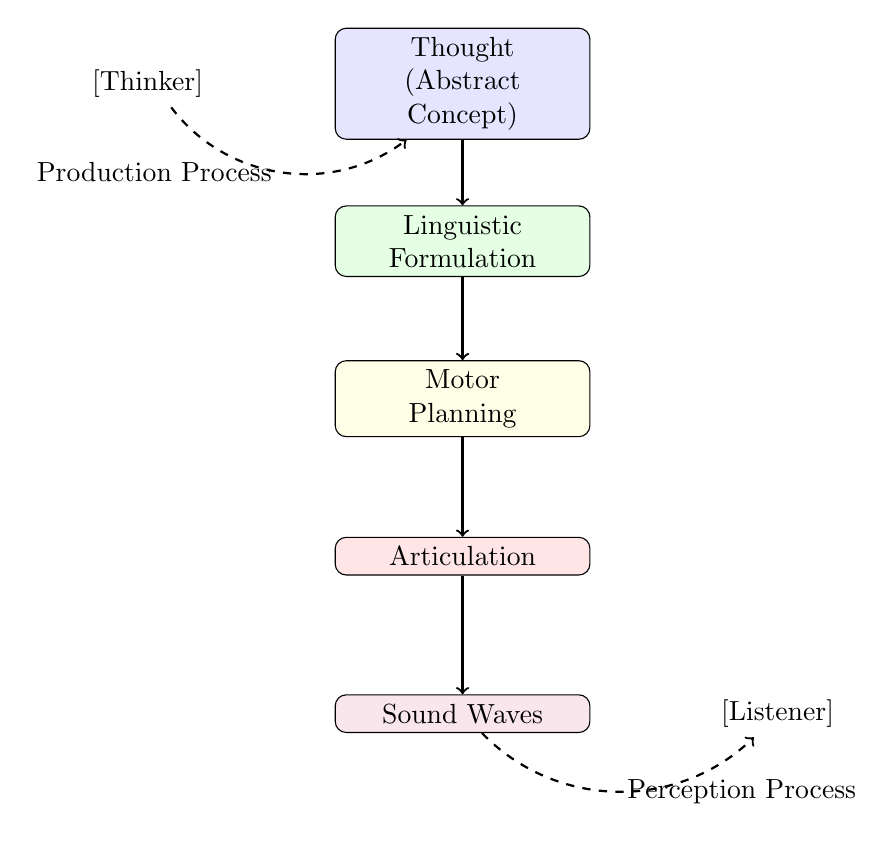
\begin{tikzpicture}[node distance=2cm, auto]
    \node [draw, rectangle, rounded corners, fill=blue!10, text width=3cm, align=center] (thought) {Thought\\(Abstract Concept)};
    \node [draw, rectangle, rounded corners, fill=green!10, text width=3cm, align=center, below of=thought] (linguistic) {Linguistic\\Formulation};
    \node [draw, rectangle, rounded corners, fill=yellow!10, text width=3cm, align=center, below of=linguistic] (motor) {Motor\\Planning};
    \node [draw, rectangle, rounded corners, fill=red!10, text width=3cm, align=center, below of=motor] (articulation) {Articulation};
    \node [draw, rectangle, rounded corners, fill=purple!10, text width=3cm, align=center, below of=articulation] (sound) {Sound Waves};
    
    \draw[->, thick] (thought) -- (linguistic);
    \draw[->, thick] (linguistic) -- (motor);
    \draw[->, thick] (motor) -- (articulation);
    \draw[->, thick] (articulation) -- (sound);
    
    \node [left of=thought, xshift=-2cm] (philosopher) {[Thinker]};
    \node [right of=sound, xshift=2cm] (listener) {[Listener]};
    
    \draw[->, thick, dashed, bend right=45] (sound) to node[right] {Perception Process} (listener);
    \draw[->, thick, dashed, bend right=45] (philosopher) to node[left] {Production Process} (thought);
\end{tikzpicture}
\caption{The journey of communication: From abstract thought to sound waves and back}
\label{fig:speech_journey}
\end{figure}

\section{The Three Realms of Speech Production: A Historical Perspective}

Speech production requires at least three fundamental mental operations, as articulated by Griffin and Ferreira (2006). These processes—conceptualization, formulation, and articulation—have parallels throughout intellectual history.

\begin{tcolorbox}[colback=green!5!white,colframe=green!75!black,title=The Speech Production Trinity]
\begin{itemize}
\item \textbf{Conceptualization} - Thinking of something to say
\item \textbf{Formulation} - Figuring out a good way to express the idea
\item \textbf{Articulation} - Moving muscles to produce sounds
\end{itemize}
\end{tcolorbox}

This tripartite division echoes philosophical frameworks across cultures and eras. In Plato's dialogue \textit{Phaedrus}, Socrates describes the process of thought formulation as requiring an understanding of truth, adaptation to the audience, and skillful delivery—paralleling our modern understanding of conceptualization, formulation, and articulation. Similarly, ancient Indian linguistic traditions distinguished between \textit{paśyantī} (pre-verbal thought), \textit{madhyamā} (mental verbalization), and \textit{vaikharī} (physical utterance).

The journey from concept to sound involves traversing boundaries between different domains of reality: from the abstract to the physical, from the private to the public, from the internal to the external. This transformation has fascinated philosophers from Aristotle to Wittgenstein, who grappled with how mental states become expressed through language.

\begin{figure}[h]
\centering
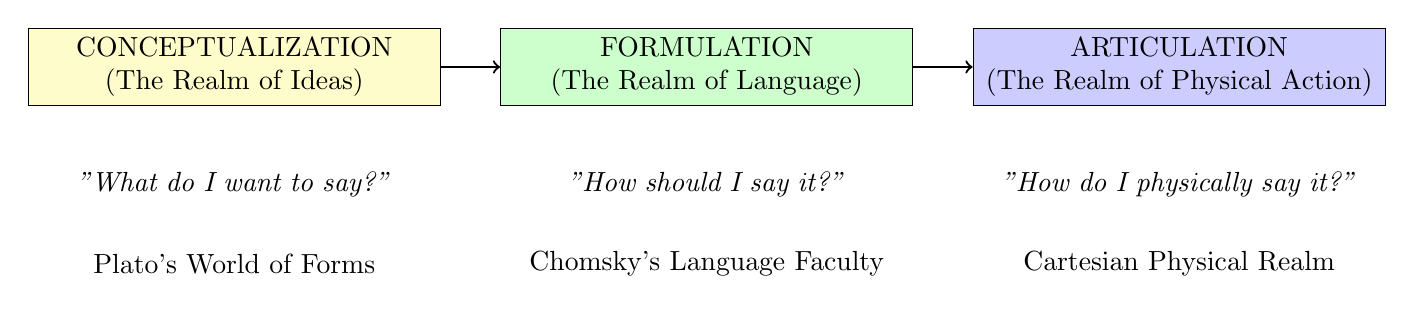
\begin{tikzpicture}
    \node[draw, fill=yellow!20, text width=5cm, align=center] (concept) at (0,0) {CONCEPTUALIZATION\\(The Realm of Ideas)};
    \node[draw, fill=green!20, text width=5cm, align=center] (form) at (6,0) {FORMULATION\\(The Realm of Language)};
    \node[draw, fill=blue!20, text width=5cm, align=center] (artic) at (12,0) {ARTICULATION\\(The Realm of Physical Action)};
    
    \draw[->, thick] (concept) -- (form);
    \draw[->, thick] (form) -- (artic);
    
    \node[text width=5cm, align=center] at (0,-1.5) {\textit{"What do I want to say?"}};
    \node[text width=5cm, align=center] at (6,-1.5) {\textit{"How should I say it?"}};
    \node[text width=5cm, align=center] at (12,-1.5) {\textit{"How do I physically say it?"}};
    
    \node[text width=5cm, align=center] at (0,-2.5) {Plato's World of Forms};
    \node[text width=5cm, align=center] at (6,-2.5) {Chomsky's Language Faculty};
    \node[text width=5cm, align=center] at (12,-2.5) {Cartesian Physical Realm};
\end{tikzpicture}
\caption{The three realms of speech production with their philosophical parallels}
\label{fig:speech_realms}
\end{figure}

\section{Levelt's Production Theory: The WEAVER++ Model}

Willem Levelt's psycholinguistic model of speech production—WEAVER++ (Word-form Encoding by Activation and VERification)—represents one of the most influential frameworks for understanding how we translate thoughts into speech. To understand this model, let us follow the journey of a thought as it becomes transformed into speech.

\begin{tcolorbox}[enhanced, frame style={upper left=yellow!75!black, upper right=green!75!black, lower left=blue!75!black, lower right=red!75!black}, interior style={top color=yellow!10, bottom color=red!10}]
Imagine a prehistoric hunter spotting a saber-toothed tiger approaching the tribe's camp. The survival of the group depends on his ability to quickly and accurately communicate this danger to others. This scenario helps illustrate the critical components of speech production as described by Levelt.
\end{tcolorbox}

\subsection{The Conceptual Preparation Stage}

Our hunter first experiences a non-linguistic mental state: the perception of danger and the recognition of a specific predator. This activates a conceptual network in his mind. This network includes not just the concept of "tiger" but associated concepts like "danger," "predator," "sharp teeth," and "running." This constellation of activated concepts constitutes the conceptual preparation stage.

Levelt proposed that this process begins with non-linguistic ideas that must connect with "lexical concepts"—ideas that have linguistic labels in a given language. This distinction helps explain a fascinating phenomenon: not all concepts can be expressed with single words in all languages. 

\begin{figure}[h]
\centering
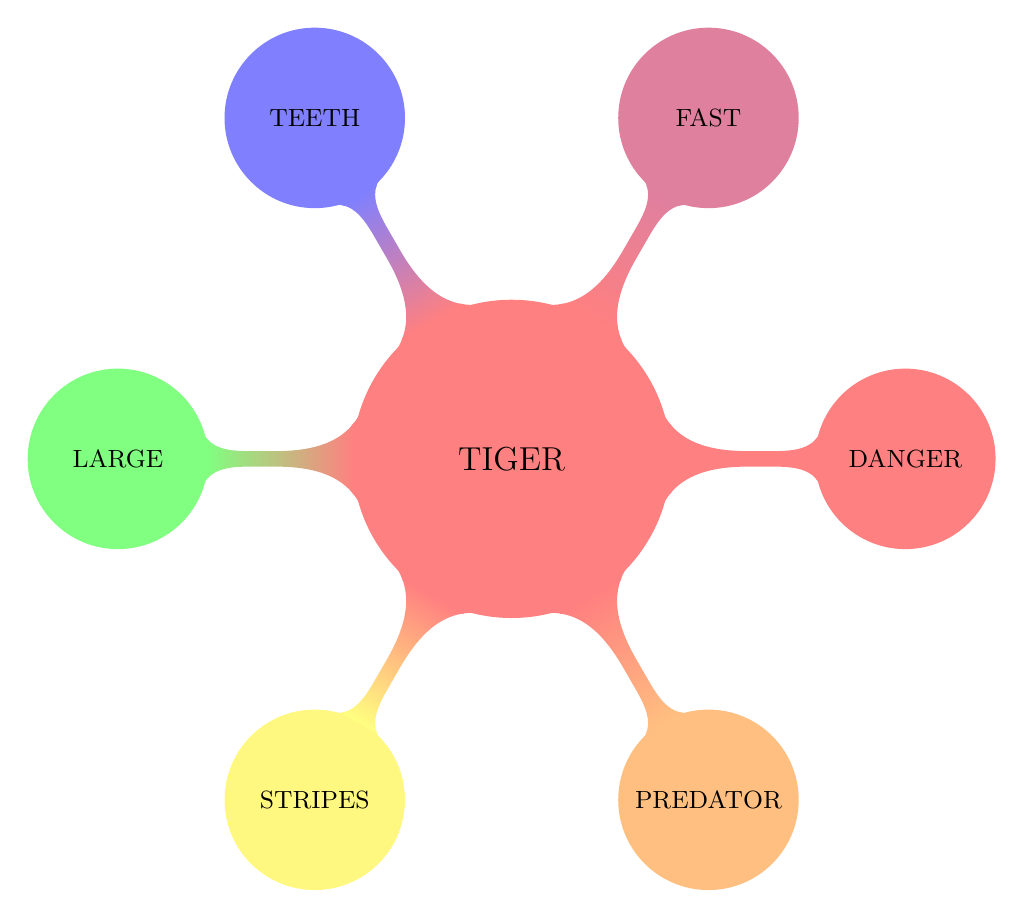
\begin{tikzpicture}[mindmap, concept color=red!50]
    \node[concept] {TIGER} [clockwise from=0]
        child[concept color=red!50] { node[concept] {DANGER} }
        child[concept color=orange!50] { node[concept] {PREDATOR} }
        child[concept color=yellow!50] { node[concept] {STRIPES} }
        child[concept color=green!50] { node[concept] {LARGE} }
        child[concept color=blue!50] { node[concept] {TEETH} }
        child[concept color=purple!50] { node[concept] {FAST} };
\end{tikzpicture}
\caption{Conceptual network activated upon seeing a tiger}
\label{fig:concept_network}
\end{figure}

For instance, as noted in Levelt's work, English has the word "mare" for a female horse but no single word for "female elephant." Similarly, the German word "Schadenfreude" (pleasure derived from another's misfortune) has no direct English equivalent. These examples illustrate how language shapes thought, a notion that resonates with the Sapir-Whorf hypothesis in linguistic anthropology.

\subsection{Lexical Selection and the Lemma}

Once lexical concepts are activated, our hunter must select specific words to express his warning. This process of lexical selection produces what Levelt calls "lemmas"—mental representations that contain information about a word's meaning and syntactic properties.

The lemma represents an intermediate stage between having an idea and producing the sounds that express that idea. It contains information about:

\begin{itemize}
\item The word's meaning
\item The word's syntactic category (noun, verb, etc.)
\item The grammatical features of the word (gender, number, tense)
\item How the word can combine with other words
\end{itemize}

\begin{table}[h]
\centering
\begin{tabular}{|l|c|c|c|}
\hline
\textbf{Lemma} & \textbf{Syntactic Category} & \textbf{Gender} & \textbf{Number} \\
\hline
tiger & noun & masculine & singular \\
run & verb & - & - \\
dangerous & adjective & - & - \\
\hline
\end{tabular}
\caption{Examples of lemma information for words in the "tiger warning" scenario}
\label{tbl:lemma_info}
\end{table}

\subsection{Morphological Encoding}

With lemmas activated, our hunter now engages in morphological encoding—determining the specific form of each word needed. Morphemes are the smallest meaningful units in language, and words can take different forms depending on their grammatical context.

For example, the lemma for "run" could be realized as "runs," "running," "ran," etc. The hunter, warning his tribe, might need to use the imperative form: "Run!" This selection process is influenced by the situational context and the grammatical structure of the intended message.

\begin{tcolorbox}[title=The Morphological Specification of "Tiger"]
\begin{center}
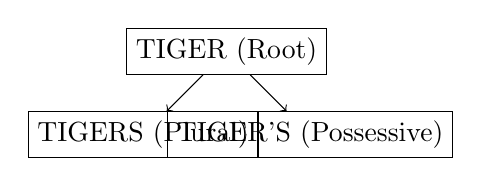
\begin{tikzpicture}[node distance=1.5cm]
    \node (tiger) [draw, rectangle] {TIGER (Root)};
    \node (tigers) [draw, rectangle, below left of=tiger] {TIGERS (Plural)};
    \node (tigers_poss) [draw, rectangle, below right of=tiger] {TIGER'S (Possessive)};
    
    \draw[->] (tiger) -- (tigers);
    \draw[->] (tiger) -- (tigers_poss);
\end{tikzpicture}
\end{center}
\end{tcolorbox}

\subsection{Phonological Encoding and Syllabification}

Now our hunter must activate the specific speech sounds (phonemes) needed to produce his warning. This process, called phonological encoding, involves:

\begin{enumerate}
\item Activating a metrical structure (the rhythmic pattern of syllables)
\item Inserting individual phonemes into the metrical structure
\item Organizing phonemes into syllables
\end{enumerate}

Levelt's key insight is that syllabification doesn't always respect word boundaries. For example, the phrase "escort us" is often pronounced as three syllables: "es-cor-tus," even though it consists of two words. This phenomenon, where the final consonant of one word joins the initial vowel of the next, is called resyllabification.

\begin{figure}[h]
\centering
\begin{tikzpicture}
    \node[draw, rounded corners, fill=blue!10] (words) at (0,0) {Word Level: \textbf{tiger coming}};
    \node[draw, rounded corners, fill=green!10] (morph) at (0,-1) {Morpheme Level: \textbf{tiger} + \textbf{com} + \textbf{ing}};
    \node[draw, rounded corners, fill=yellow!10] (syll) at (0,-2) {Syllable Level: \textbf{ti} + \textbf{ger} + \textbf{co} + \textbf{ming}};
    \node[draw, rounded corners, fill=red!10] (phono) at (0,-3) {Phoneme Level: /t/ /aɪ/ /g/ /ər/ /k/ /ʌ/ /m/ /ɪ/ /ŋ/};
    
    \draw[->] (words) -- (morph);
    \draw[->] (morph) -- (syll);
    \draw[->] (syll) -- (phono);
\end{tikzpicture}
\caption{Hierarchical encoding from words to phonemes}
\label{fig:phono_encoding}
\end{figure}

\subsection{Phonetic Encoding and Articulation}

Finally, our hunter must execute the physical movements required to produce the warning. Levelt proposed that speakers access a "mental syllabary"—a store of memorized motor programs for frequently used syllables. These motor programs guide the complex coordination of over 100 muscles involved in speech production.

The result is a "phonetic gestural score"—essentially, a detailed plan for how to move the articulators (tongue, lips, vocal cords) to produce the intended sounds. This plan is then executed by the motor system, creating the sound waves that will convey the warning to the hunter's tribe members.

\begin{tcolorbox}[enhanced, frame style={red!75!black}, interior style={red!10}]
Remarkably, all these processes unfold in mere milliseconds. From the moment our prehistoric hunter spots the tiger to his shouted warning takes less than a second, yet involves a cascade of mental operations spanning conceptual, linguistic, and motor domains.
\end{tcolorbox}

\section{Evidence from Speech Errors: Windows into the Mind}

Speech errors—or "slips of the tongue"—provide fascinating evidence for models like Levelt's WEAVER++. Where Sigmund Freud saw these errors as revelations of suppressed thoughts, modern psycholinguists view them as systematic breakdowns in speech production processes.

\subsection{The Taxonomy of Speech Errors}

Speech errors follow systematic patterns that reveal the architecture of the production system. Consider these categories:

\begin{table}[h]
\centering
\begin{tabular}{|p{3cm}|p{5cm}|p{5cm}|}
\hline
\textbf{Error Type} & \textbf{Example} & \textbf{Process Revealed} \\
\hline
Semantic substitution & Saying "dog" instead of "cat" & Conceptual preparation / Lexical selection \\
\hline
Sound exchange & "Fig beet" instead of "big feet" & Phonological encoding \\
\hline
Word exchange & "My piano plays the girlfriend" instead of "My girlfriend plays the piano" & Syntactic frame construction \\
\hline
\end{tabular}
\caption{Types of speech errors and their implications}
\label{tbl:error_types}
\end{table}

\subsection{The Positional Constraint: Order in Chaos}

One fascinating aspect of sound exchange errors is that they typically respect position—sounds usually trade places with other sounds from the same position in different words. For example, a speaker might say "bad mack" instead of "mad back," swapping initial consonants.

This positional constraint provides evidence for Dell's frame-and-slot model, where phonemes are tagged with position information (first, middle, last) and inserted into syllable frames. Errors occur when phonemes with the same position tag get misdirected, but the system rarely jams a "first position" phoneme into a "last position" slot.

\begin{figure}[h]
\centering
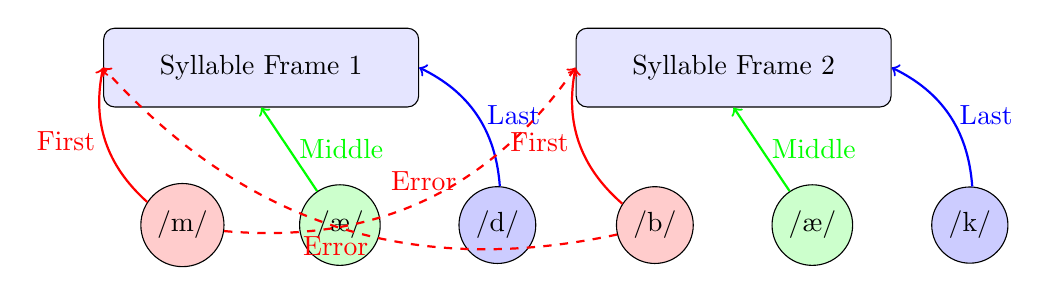
\begin{tikzpicture}
    \node[draw, rounded corners, fill=blue!10, minimum width=4cm, minimum height=1cm] (frame1) at (0,0) {Syllable Frame 1};
    \node[draw, rounded corners, fill=blue!10, minimum width=4cm, minimum height=1cm] (frame2) at (6,0) {Syllable Frame 2};
    
    \node[draw, circle, fill=red!20] (ph1) at (-1,-2) {/m/};
    \node[draw, circle, fill=green!20] (ph2) at (1,-2) {/æ/};
    \node[draw, circle, fill=blue!20] (ph3) at (3,-2) {/d/};
    
    \node[draw, circle, fill=red!20] (ph4) at (5,-2) {/b/};
    \node[draw, circle, fill=green!20] (ph5) at (7,-2) {/æ/};
    \node[draw, circle, fill=blue!20] (ph6) at (9,-2) {/k/};
    
    \draw[->, thick, color=red] (ph1) to[bend left] node[midway, left] {First} (frame1.180);
    \draw[->, thick, color=green] (ph2) to node[midway, right] {Middle} (frame1.270);
    \draw[->, thick, color=blue] (ph3) to[bend right] node[midway, right] {Last} (frame1.0);
    
    \draw[->, thick, color=red] (ph4) to[bend left] node[midway, left] {First} (frame2.180);
    \draw[->, thick, color=green] (ph5) to node[midway, right] {Middle} (frame2.270);
    \draw[->, thick, color=blue] (ph6) to[bend right] node[midway, right] {Last} (frame2.0);
    
    \draw[->, thick, dashed, color=red] (ph1) to[bend right] node[midway, above] {Error} (frame2.180);
    \draw[->, thick, dashed, color=red] (ph4) to[bend left] node[midway, below] {Error} (frame1.180);
\end{tikzpicture}
\caption{Position-constrained phoneme errors: /m/ and /b/ can exchange because both have "first position" tags}
\label{fig:position_constraint}
\end{figure}

\subsection{The Category Constraint: Like Exchanges with Like}

Word exchange errors typically respect syntactic categories—a noun exchanges with another noun, a verb with another verb. This provides evidence for syntactic frame construction in speech planning, where slots are labeled for specific word types (noun, verb, adjective).

As the psycholinguist Merrill Garrett observed in 1975, this suggests we plan speech in larger units than individual words, laying out syntactic structures before filling them with specific lexical items—similar to how one might fill in a Mad Libs game with words of the correct grammatical category.

\begin{tcolorbox}[title=The Category Constraint in Action]
\begin{center}
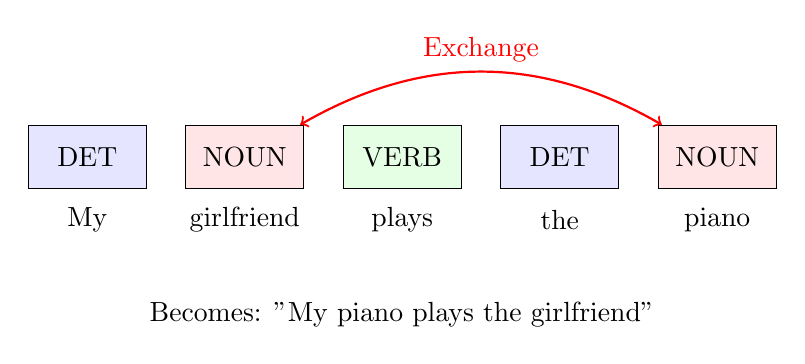
\begin{tikzpicture}
    \node[draw, rectangle, fill=blue!10, minimum width=1.5cm, minimum height=0.8cm] (det1) at (0,0) {DET};
    \node[draw, rectangle, fill=red!10, minimum width=1.5cm, minimum height=0.8cm] (n1) at (2,0) {NOUN};
    \node[draw, rectangle, fill=green!10, minimum width=1.5cm, minimum height=0.8cm] (v) at (4,0) {VERB};
    \node[draw, rectangle, fill=blue!10, minimum width=1.5cm, minimum height=0.8cm] (det2) at (6,0) {DET};
    \node[draw, rectangle, fill=red!10, minimum width=1.5cm, minimum height=0.8cm] (n2) at (8,0) {NOUN};
    
    \node at (0,-0.8) {My};
    \node at (2,-0.8) {girlfriend};
    \node at (4,-0.8) {plays};
    \node at (6,-0.8) {the};
    \node at (8,-0.8) {piano};
    
    \draw[<->, thick, bend left=30, color=red] (n1) to node[midway, above] {Exchange} (n2);
    
    \node at (4,-2) {Becomes: "My piano plays the girlfriend"};
\end{tikzpicture}
\end{center}
\end{tcolorbox}

\section{The Tip-of-the-Tongue Phenomenon: Memory at the Threshold}

The tip-of-the-tongue (TOT) state represents a fascinating window into speech production processes. This experience—where we feel we know a word but cannot retrieve it—has captivated philosophers and psychologists for centuries.

\subsection{The Historical Context of TOT Research}

William James described this phenomenon in his 1890 work \textit{Principles of Psychology}: "The state of our consciousness is peculiar. There is a gap therein; but no mere gap. It is a gap that is intensely active." This description captures the frustrating yet active nature of the TOT state—we know something is there, yet cannot grasp it.

Systematic research on TOT began with Roger Brown and David McNeill's 1966 study, where they induced TOT states by asking participants to name objects from definitions. Their findings suggested that during TOT states, people often have partial access to phonological information about the target word.

\begin{figure}[h]
\centering
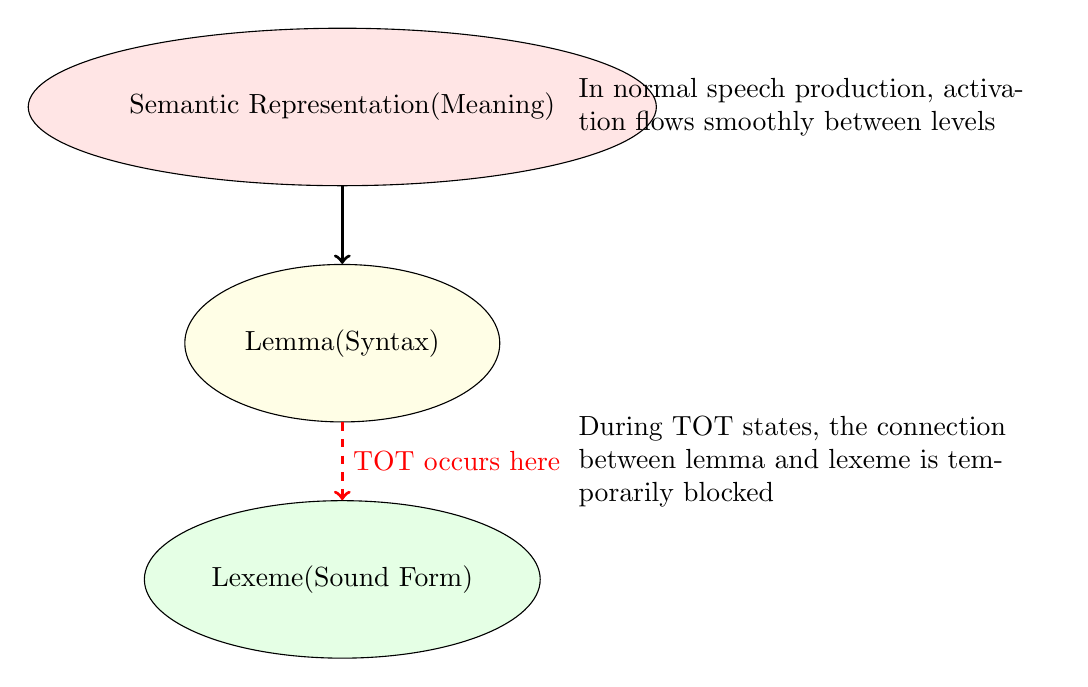
\begin{tikzpicture}
    \node[draw, ellipse, fill=red!10, minimum width=4cm, minimum height=2cm] (semantic) at (0,0) {Semantic Representation\\(Meaning)};
    \node[draw, ellipse, fill=yellow!10, minimum width=4cm, minimum height=2cm] (lemma) at (0,-3) {Lemma\\(Syntax)};
    \node[draw, ellipse, fill=green!10, minimum width=4cm, minimum height=2cm] (lexeme) at (0,-6) {Lexeme\\(Sound Form)};
    
    \draw[->, very thick] (semantic) -- (lemma);
    \draw[->, very thick, dashed, color=red] (lemma) -- node[right] {TOT occurs here} (lexeme);
    
    \node[text width=6cm] at (6,0) {In normal speech production, activation flows smoothly between levels};
    \node[text width=6cm] at (6,-4.5) {During TOT states, the connection between lemma and lexeme is temporarily blocked};
\end{tikzpicture}
\caption{The Tip-of-the-Tongue phenomenon as a breakdown between lemma and lexeme levels}
\label{fig:tot_phenomenon}
\end{figure}

\subsection{TOT as Evidence for Production Models}

TOT phenomena strongly support two-stage models of lexical access like Levelt's. During a TOT state, we have successfully activated the lemma (we know the word's meaning and grammatical properties) but cannot fully activate the lexeme (the word's sound pattern).

Evidence for this interpretation comes from several observations:

\begin{enumerate}
\item People experiencing TOT can accurately predict whether they will eventually retrieve the word
\item They often know the number of syllables in the target word
\item They can frequently identify the first letter or sound
\item They tend to retrieve words that sound similar to the target
\end{enumerate}

This reveals that during TOT, substantial phonological information is partially activated, but not sufficiently to produce the word. As the psychologist Bennett Schwartz noted, TOT states are "windows into the architecture of the lexical retrieval system."

\subsection{The Universal Experience Across Cultures}

TOT states appear to be universal across languages and cultures. Studies in Mandarin Chinese, Russian, Italian, and dozens of other languages reveal similar phenomenology. This universality suggests TOT reflects fundamental properties of human memory and language processing rather than language-specific quirks.

However, the frequency of TOT experiences increases with age, suggesting changes in lexical access across the lifespan—a finding that connects psycholinguistics with the study of cognitive aging.

\begin{tcolorbox}[enhanced, colback=purple!5, colframe=purple!75!black, title=Phenomenology of TOT States]
Imagine trying to recall the name of an actor. During a TOT state, you might experience:

\begin{itemize}
\item A strong feeling that you know the name
\item The sensation that the name is "just out of reach"
\item Knowledge that the name starts with "B"
\item Awareness that it has three syllables
\item The ability to recall similar-sounding names
\end{itemize}

This partial access to phonological information is precisely what we would expect if the semantic and syntactic information (lemma) has been successfully activated, but the phonological form (lexeme) remains partially inaccessible.
\end{tcolorbox}

\section{Picture-Naming Studies: Experimental Windows into Production}

Picture-naming paradigms have provided crucial evidence about speech production processes since the pioneering work of Oldfield and Wingfield in 1965. These seemingly simple tasks—asking participants to name objects in images—reveal the complex operations underlying word retrieval and production.

\subsection{The Historical Development of Picture-Naming Methods}

The use of picture naming in psycholinguistic research represents an example of how simple experimental paradigms can yield profound insights. Early studies revealed that while object recognition times are minimally affected by an object's familiarity, naming times show strong frequency effects—less frequently used words take longer to produce than common words.

This dissociation between recognition and naming provides evidence for separate processes in object identification and name retrieval—a distinction that parallels the separation between conceptual preparation and lexical selection in Levelt's model.

\begin{figure}[h]
\centering
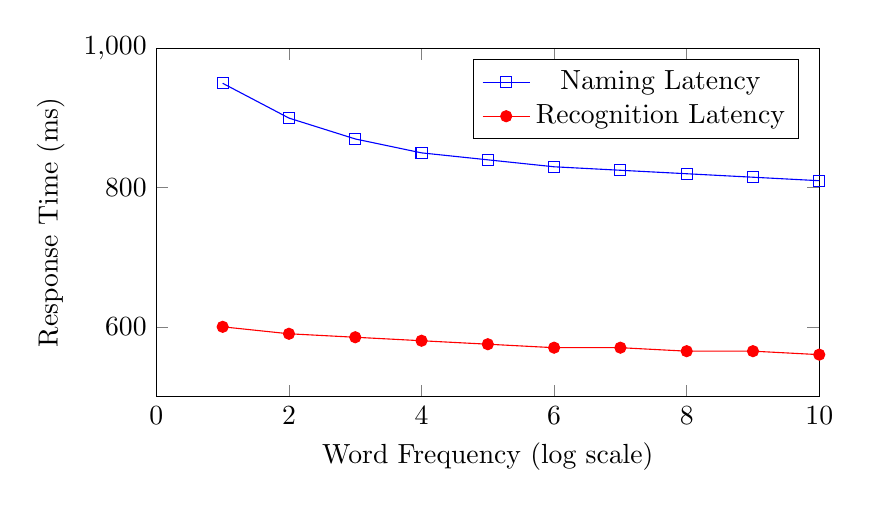
\begin{tikzpicture}
    \begin{axis}[
        width=10cm,
        height=6cm,
        xlabel=Word Frequency (log scale),
        ylabel=Response Time (ms),
        legend pos=north east,
        ymin=500, ymax=1000,
        xmin=0, xmax=10
    ]
    
    \addplot[
        color=blue,
        mark=square,
    ] coordinates {
        (1, 950)
        (2, 900)
        (3, 870)
        (4, 850)
        (5, 840)
        (6, 830)
        (7, 825)
        (8, 820)
        (9, 815)
        (10, 810)
    };
    
    \addplot[
        color=red,
        mark=*,
    ] coordinates {
        (1, 600)
        (2, 590)
        (3, 585)
        (4, 580)
        (5, 575)
        (6, 570)
        (7, 570)
        (8, 565)
        (9, 565)
        (10, 560)
    };
    
    \legend{Naming Latency, Recognition Latency}
    
    \end{axis}
\end{tikzpicture}
\caption{Word frequency effects on naming versus recognition latencies}
\label{fig:naming_latencies}
\end{figure}

\subsection{The Picture-Word Interference Paradigm}

A crucial variant of the picture-naming task is the picture-word interference paradigm, where participants name pictures with superimposed words. This creates competition between the picture name and the distractor word, allowing researchers to probe different stages of lexical access.

Three key conditions in picture-word interference studies reveal the architecture of the production system:

\begin{enumerate}
\item \textbf{Identity condition:} The superimposed word is identical to the picture name (e.g., picture of a house, word "house")
\item \textbf{Semantic condition:} The superimposed word is semantically related to the picture (e.g., picture of a house, word "building")
\item \textbf{Phonological condition:} The superimposed word sounds similar to the picture name (e.g., picture of a house, word "mouse")
\end{enumerate}

The pattern of results—semantic interference but phonological facilitation—provides compelling evidence for distinct semantic and phonological stages in lexical access.

\begin{tcolorbox}[enhanced, colback=green!5, colframe=green!75!black, title=Experimental Evidence: Semantic Interference vs. Phonological Facilitation]
\begin{center}
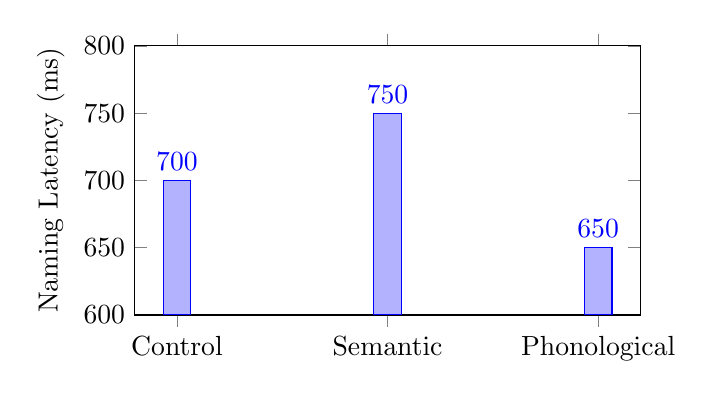
\begin{tikzpicture}
    \begin{axis}[
        width=8cm,
        height=5cm,
        ylabel=Naming Latency (ms),
        symbolic x coords={Control, Semantic, Phonological},
        xtick=data,
        ybar,
        ymin=600, ymax=800,
        nodes near coords,
    ]
    \addplot coordinates {(Control, 700) (Semantic, 750) (Phonological, 650)};
    \end{axis}
\end{tikzpicture}
\end{center}

When naming a picture of a dog:
\begin{itemize}
\item Control condition (unrelated word "table"): 700ms
\item Semantic condition (related word "cat"): 750ms (interference)
\item Phonological condition (similar-sounding "log"): 650ms (facilitation)
\end{itemize}
\end{tcolorbox}

\section{Competing Models: WEAVER++ vs. Spreading Activation}

While Levelt's WEAVER++ model assumes a strict feed-forward flow of information, Dell's spreading activation model proposes a more interactive architecture with bidirectional connections between levels. This fundamental difference in information flow leads to different predictions about speech production phenomena.

\subsection{The Philosophical Context: Feed-Forward vs. Interactive Processing}

The debate between strict feed-forward and interactive models connects to broader questions in cognitive science and philosophy of mind. Feed-forward models align with modular views of cognition (as championed by Jerry Fodor), where specialized processors operate independently with minimal cross-talk. Interactive models align with more connectionist approaches, emphasizing the brain's densely interconnected nature.

This scientific debate echoes ancient philosophical tensions between atomistic views of mind (where mental processes consist of independent operations) and holistic perspectives (where mental processes form an interconnected web).

\begin{figure}[h]
\centering
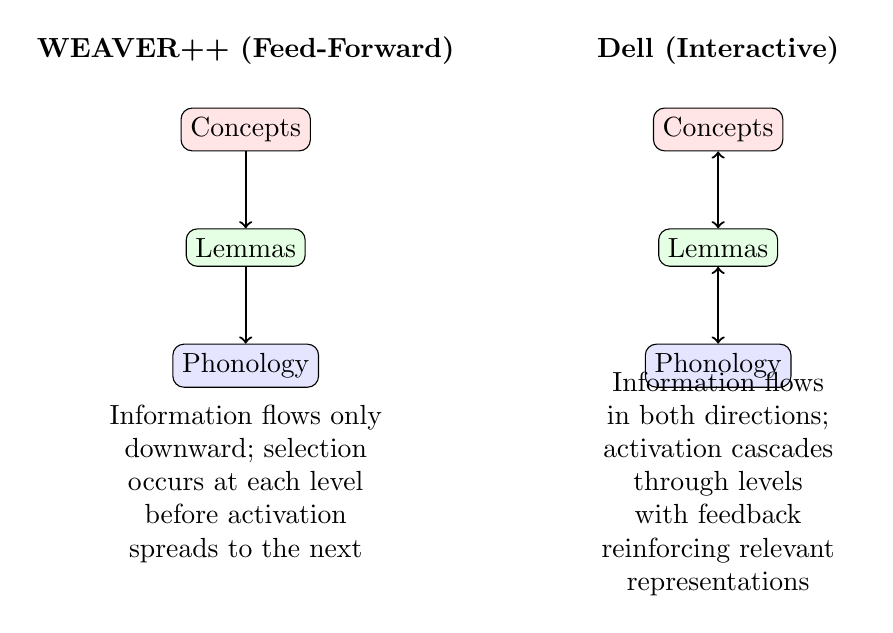
\begin{tikzpicture}[node distance=2.5cm]
    \node (title1) at (0,0) {\textbf{WEAVER++ (Feed-Forward)}};
    \node (title2) at (6,0) {\textbf{Dell (Interactive)}};
    
    \node[draw, rectangle, rounded corners, fill=red!10] (c1) at (0,-1) {Concepts};
    \node[draw, rectangle, rounded corners, fill=green!10] (l1) at (0,-2.5) {Lemmas};
    \node[draw, rectangle, rounded corners, fill=blue!10] (p1) at (0,-4) {Phonology};
    
    \node[draw, rectangle, rounded corners, fill=red!10] (c2) at (6,-1) {Concepts};
    \node[draw, rectangle, rounded corners, fill=green!10] (l2) at (6,-2.5) {Lemmas};
    \node[draw, rectangle, rounded corners, fill=blue!10] (p2) at (6,-4) {Phonology};
    
    \draw[->, thick] (c1) -- (l1);
    \draw[->, thick] (l1) -- (p1);
    
    \draw[<->, thick] (c2) -- (l2);
    \draw[<->, thick] (l2) -- (p2);
    
    \node[text width=3.5cm, align=center] at (0,-5.5) {Information flows only downward; selection occurs at each level before activation spreads to the next};
    
    \node[text width=3.5cm, align=center] at (6,-5.5) {Information flows in both directions; activation cascades through levels with feedback reinforcing relevant representations};
\end{tikzpicture}
\caption{Contrasting information flow in WEAVER++ and Dell's spreading activation models}
\label{fig:model_comparison}
\end{figure}

\subsection{Explaining the Lexical Bias Effect}

One key phenomenon that distinguishes these models is the lexical bias effect—the tendency for sound errors to create real words more often than would be expected by chance. For instance, speakers are more likely to say "barn door" as "darn bore" (both real words) than as "darn boor" (where "boor" is less common).

The interactive spreading activation model explains this through feedback connections. When phonological units are activated, they send activation back to the lemma level. Because real words have lemma representations and non-words don't, sound patterns that would create real words receive additional activation through this feedback loop.

\begin{tcolorbox}[enhanced, colback=blue!5, colframe=blue!75!black, title=The Lexical Bias Effect Explained]
\begin{center}
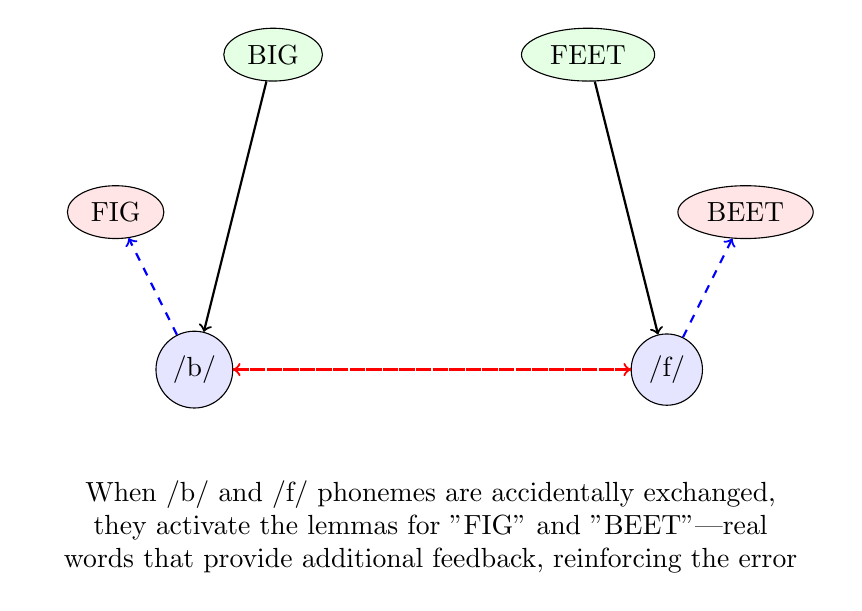
\begin{tikzpicture}
    \node[draw, ellipse, fill=green!10] (word1) at (0,0) {BIG};
    \node[draw, ellipse, fill=green!10] (word2) at (4,0) {FEET};
    
    \node[draw, ellipse, fill=red!10] (fig) at (-2,-2) {FIG};
    \node[draw, ellipse, fill=red!10] (beet) at (6,-2) {BEET};
    
    \node[draw, circle, fill=blue!10] (b) at (-1,-4) {/b/};
    \node[draw, circle, fill=blue!10] (f) at (5,-4) {/f/};
    
    \draw[->, thick] (word1) -- (b);
    \draw[->, thick] (word2) -- (f);
    
    \draw[->, thick, dashed, color=red] (b) -- (f.west);
    \draw[->, thick, dashed, color=red] (f) -- (b.east);
    
    \draw[->, thick, dashed, color=blue, bend right] (b) -- (fig);
    \draw[->, thick, dashed, color=blue, bend left] (f) -- (beet);
    
    \node[text width=10cm, align=center] at (2,-6) {When /b/ and /f/ phonemes are accidentally exchanged, they activate the lemmas for "FIG" and "BEET"—real words that provide additional feedback, reinforcing the error};
\end{tikzpicture}
\end{center}
\end{tcolorbox}

\subsection{Mixed Errors: The Challenge to Feed-Forward Models}

Mixed errors—where a word is substituted with another word that is both semantically and phonologically related to the target—present a challenge to strict feed-forward models. For example, saying "lobster" instead of "oyster" (related in both meaning and sound) occurs more frequently than chance would predict.

Dell's interactive model explains mixed errors through cascading activation and feedback:
\begin{enumerate}
\item Thinking about "oyster" activates semantically related concepts like "lobster"
\item Both lemmas send activation to their phonological units
\item The shared phonological elements (/stər/) receive doubled activation
\item Feedback from these phonological units further reinforces the "lobster" lemma
\end{enumerate}

Without cascading activation and feedback, there is no clear mechanism for producing the observed pattern of mixed errors.

\section{From Theory to Brain: Neuropsychological Evidence}

Alfonso Caramazza's critique of lemma theory based on neuropsychological evidence represents an important challenge to both the WEAVER++ and spreading activation accounts. His observations of patients with brain damage reveal patterns that are difficult to reconcile with a single lemma level.

\subsection{The Historical Context of Neuropsychological Research}

The tradition of using neurological disorders to understand language processing dates back to the 19th century work of Paul Broca and Carl Wernicke, who identified specific brain regions associated with speech production and comprehension, respectively. The dissociation between production and comprehension deficits provided early evidence for specialized language systems in the brain.

Caramazza's research extends this tradition, using double dissociations in patient populations to test specific claims about the architecture of the language production system.

\begin{figure}[h]
\centering
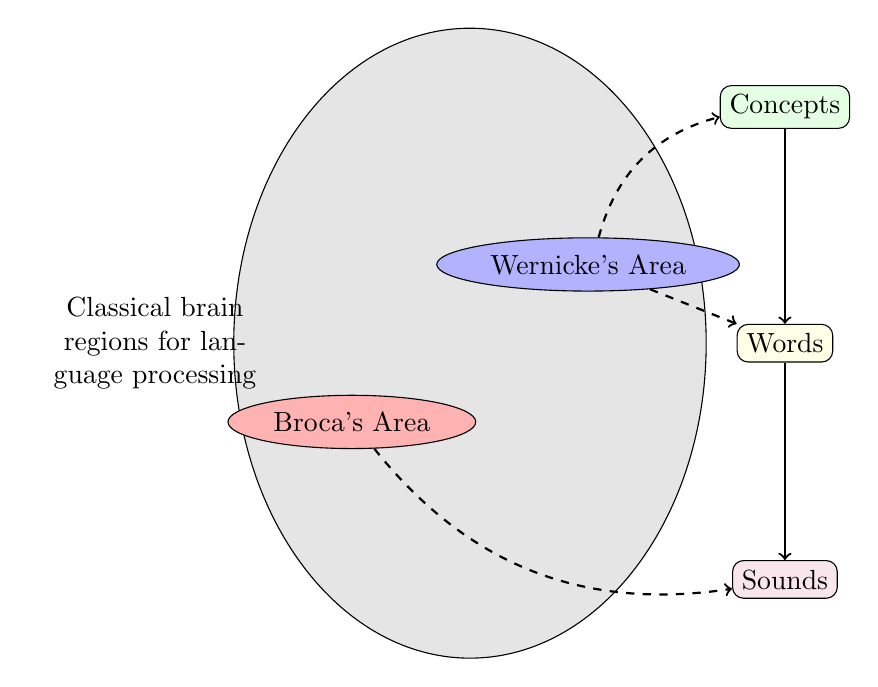
\begin{tikzpicture}
    \node[draw, ellipse, fill=gray!20, minimum width=6cm, minimum height=8cm] (brain) at (0,0) {};
    
    \node[draw, ellipse, fill=red!30] (broca) at (-1.5,-1) {Broca's Area};
    \node[draw, ellipse, fill=blue!30] (wernicke) at (1.5,1) {Wernicke's Area};
    
    \node[draw, rectangle, rounded corners, fill=green!10] (concepts) at (4,3) {Concepts};
    \node[draw, rectangle, rounded corners, fill=yellow!10] (words) at (4,0) {Words};
    \node[draw, rectangle, rounded corners, fill=purple!10] (sounds) at (4,-3) {Sounds};
    
    \draw[->, thick] (concepts) -- (words);
    \draw[->, thick] (words) -- (sounds);
    
    \draw[->, thick, dashed] (wernicke) to[bend left] (concepts);
    \draw[->, thick, dashed] (wernicke) to (words);
    \draw[->, thick, dashed] (broca) to[bend right] (sounds);
    
    \node[text width=3cm, align=center] at (-4,0) {Classical brain regions for language processing};
    
\end{tikzpicture}
\caption{Simplified view of language regions in the brain and their relationship to production stages}
\label{fig:brain_language}
\end{figure}

\subsection{The Challenge from Modality-Specific Deficits}

Caramazza discovered patients with fascinating patterns of language impairment. Some showed selective difficulties with specific word types (content vs. function words) that varied depending on the output modality—speaking versus writing.

For example, a patient might struggle with function words (like "the" or "and") when writing but have problems with content words (like "tiger" or "house") when speaking. If both speaking and writing access the same lemma representations, such dissociations should be impossible.

\begin{table}[h]
\centering
\begin{tabular}{|c|c|c|}
\hline
\textbf{Patient Type} & \textbf{Speaking Deficit} & \textbf{Writing Deficit} \\
\hline
Patient A & Content words & Function words \\
\hline
Patient B & Function words & Content words \\
\hline
\end{tabular}
\caption{Double dissociations in patients with brain damage}
\label{tbl:patient_dissociations}
\end{table}

Similarly, Caramazza documented patients who produced different semantic errors depending on output modality—consistently saying "dish" when trying to name a picture of a cook but writing "forks" when asked to write the name.

\subsection{The Independent Network Model: An Alternative Account}

To explain these findings, Caramazza proposed the "Independent Network" model, which posits:

\begin{itemize}
\item Separate lexical-form networks for spoken and written language
\item Grammatical information stored separately from word forms
\item Direct connections between semantic and phonological/orthographic representations without an intervening lemma level
\end{itemize}

This model accounts for the observed double dissociations but challenges the fundamental architecture of both WEAVER++ and spreading activation models.

\begin{figure}[h]
\centering
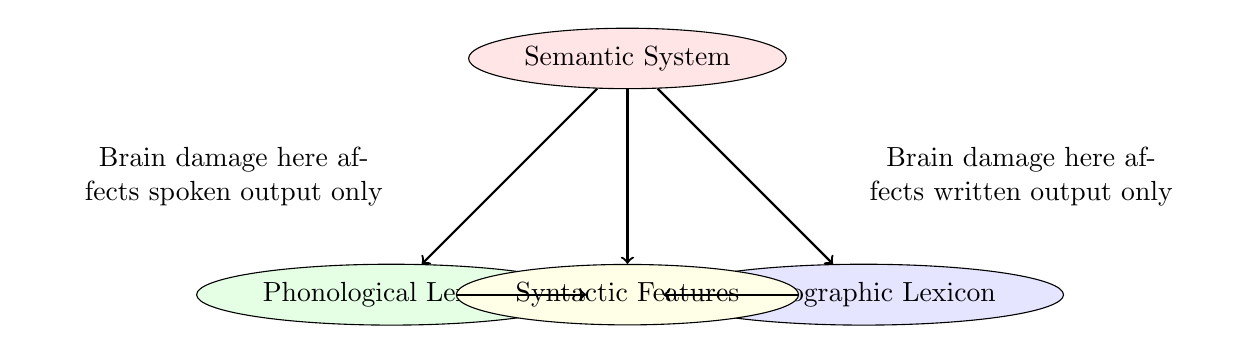
\begin{tikzpicture}
    \node[draw, ellipse, fill=red!10] (semantic) at (0,0) {Semantic System};
    
    \node[draw, ellipse, fill=green!10] (phonological) at (-3,-3) {Phonological Lexicon};
    \node[draw, ellipse, fill=blue!10] (orthographic) at (3,-3) {Orthographic Lexicon};
    \node[draw, ellipse, fill=yellow!10] (syntactic) at (0,-3) {Syntactic Features};
    
    \draw[->, thick] (semantic) -- (phonological);
    \draw[->, thick] (semantic) -- (orthographic);
    \draw[->, thick] (semantic) -- (syntactic);
    \draw[->, thick] (syntactic) -- (phonological);
    \draw[->, thick] (syntactic) -- (orthographic);
    
    \node[text width=5cm, align=center] at (-5,-1.5) {Brain damage here affects spoken output only};
    \node[text width=5cm, align=center] at (5,-1.5) {Brain damage here affects written output only};
\end{tikzpicture}
\caption{Caramazza's Independent Network model}
\label{fig:independent_network}
\end{figure}

\section{The Final Frontier: Articulation and Speech Perception}

\subsection{Articulation: The Bridge Between Mind and Sound}

Ultimately, speech production culminates in articulation—the physical movements that create sound waves. This process involves configuring the vocal tract through coordinated movements of the lips, tongue, vocal folds, and other articulators.

Articulatory phonology (developed by Browman and Goldstein) classifies speech sounds according to gestures rather than abstract phonological features. This approach focuses on the movements of articulators:

\begin{itemize}
\item The lips
\item The tongue tip
\item The tongue body
\item The velum (soft palate)
\item The glottis (housing the vocal folds)
\end{itemize}

\begin{figure}[h]
\centering
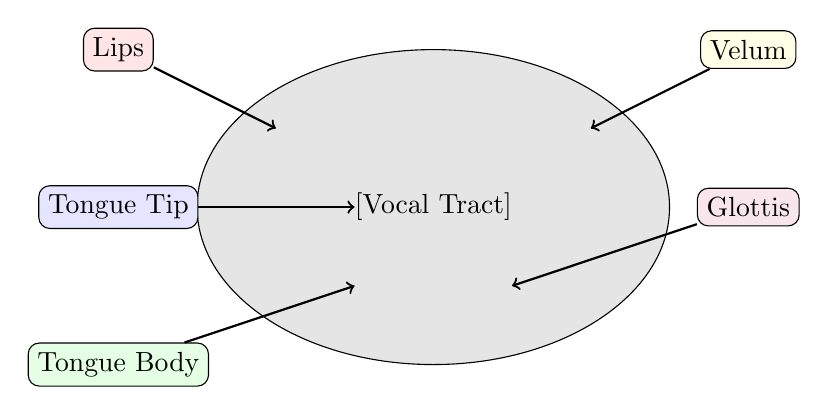
\begin{tikzpicture}
    \node[draw, ellipse, fill=gray!20, minimum width=6cm, minimum height=4cm] (vocal) at (0,0) {[Vocal Tract]};
    
    \node[draw, rectangle, rounded corners, fill=red!10] (lips) at (-4,2) {Lips};
    \node[draw, rectangle, rounded corners, fill=blue!10] (tongue_tip) at (-4,0) {Tongue Tip};
    \node[draw, rectangle, rounded corners, fill=green!10] (tongue_body) at (-4,-2) {Tongue Body};
    \node[draw, rectangle, rounded corners, fill=yellow!10] (velum) at (4,2) {Velum};
    \node[draw, rectangle, rounded corners, fill=purple!10] (glottis) at (4,0) {Glottis};
    
    \draw[->, thick] (lips) -- (-2,1);
    \draw[->, thick] (tongue_tip) -- (-1,0);
    \draw[->, thick] (tongue_body) -- (-1,-1);
    \draw[->, thick] (velum) -- (2,1);
    \draw[->, thick] (glottis) -- (1,-1);
\end{tikzpicture}
\caption{The articulators involved in speech production}
\label{fig:articulators}
\end{figure}

\subsection{Coarticulation: Efficiency in Speech Production}

One of the most remarkable aspects of speech production is coarticulation—the overlap of articulatory gestures for different phonemes. Rather than producing one phoneme at a time in sequence, we blend the movements, with gestures for one phoneme beginning while those for the previous phoneme are still underway.

This phenomenon helps explain how humans achieve the remarkable speed of conversational speech—about 15 phonemes per second. Without coarticulation, speech would be dramatically slower and require far more effort.

\begin{tcolorbox}[enhanced, colback=orange!5, colframe=orange!75!black, title=Coarticulation: The Blending of Gestures]
When saying the word "pool":
\begin{itemize}
\item As you position your lips to pronounce the /p/, you're already rounding them in anticipation of the /u/ sound
\item Your tongue is already positioning for the /l/ even as you're articulating the /u/
\end{itemize}

This overlap in articulation creates a more efficient speech stream but means that the acoustic signal for each phoneme is heavily influenced by neighboring phonemes—a phenomenon that creates challenges for speech perception.
\end{tcolorbox}

\subsection{The Motor Theory of Speech Perception}

The Motor Theory of Speech Perception, developed by Alvin Liberman and colleagues at Haskins Laboratories, proposes that we understand speech by reference to the articulatory gestures that produced it, rather than by analyzing the acoustic signal directly.

This theory emerged from a fundamental observation: the acoustic patterns that correspond to phonemes are highly variable depending on context. For example, the /d/ sound in "di" and "du" produces radically different acoustic patterns, yet listeners perceive the same consonant in both syllables.

\begin{figure}[h]
\centering
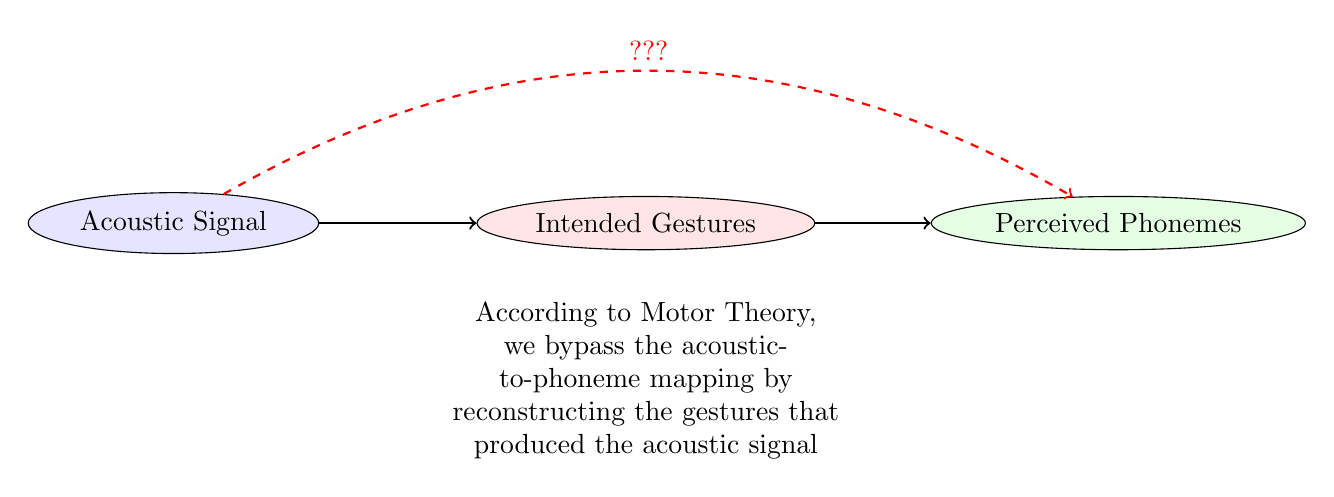
\begin{tikzpicture}
    \node[draw, ellipse, fill=blue!10] (acoustic) at (0,0) {Acoustic Signal};
    \node[draw, ellipse, fill=red!10] (intended) at (6,0) {Intended Gestures};
    \node[draw, ellipse, fill=green!10] (phonemes) at (12,0) {Perceived Phonemes};
    
    \draw[->, thick, dashed, color=red] (acoustic) to[bend left] node[above] {???} (phonemes);
    \draw[->, thick] (acoustic) -- (intended);
    \draw[->, thick] (intended) -- (phonemes);
    
    \node[text width=5cm, align=center] at (6,-2) {According to Motor Theory, we bypass the acoustic-to-phoneme mapping by reconstructing the gestures that produced the acoustic signal};
\end{tikzpicture}
\caption{The indirect perception pathway proposed by Motor Theory}
\label{fig:motor_theory}
\end{figure}

Key phenomena supporting Motor Theory include:

\begin{enumerate}
\item \textbf{Categorical perception:} Listeners perceive speech sounds categorically rather than continuously, even though the acoustic signals vary continuously
\item \textbf{The McGurk Effect:} Visual information about articulatory gestures can override acoustic information in speech perception
\item \textbf{Duplex perception:} The same acoustic element can be perceived as a chirp when isolated and as a phoneme when in a speech context
\end{enumerate}

\subsection{Mirror Neurons and the Neural Basis of Speech Perception}

Recent discoveries about mirror neurons—cells that fire both when an animal performs an action and when it observes the same action—have revitalized interest in Motor Theory. Researchers have proposed that a mirror neuron system in Broca's area may provide the neural mechanism for mapping between perceived speech and the motor representations used in speech production.

Evidence supporting this view comes from neuroimaging studies showing that listening to speech activates motor regions involved in speech production. For example, hearing syllables with bilabial stops (/pa/, /ba/) activates different motor cortex regions than hearing syllables with alveolar stops (/ta/, /da/).

\begin{tcolorbox}[enhanced, colback=purple!5, colframe=purple!75!black, title=Mirror Neurons: A Modern Perspective on Motor Theory]
The discovery of mirror neurons by Gallese and colleagues (1996) offered a potential neural mechanism for Motor Theory:

\begin{itemize}
\item Mirror neurons in macaque monkeys fire both when performing an action and when observing the same action
\item Human neuroimaging studies show activity in motor regions during speech perception
\item TMS applied to tongue regions of motor cortex affects perception of tongue-related phonemes
\end{itemize}

These findings suggest motor representations may indeed play a role in speech perception, though perhaps not exactly as Liberman originally proposed.
\end{tcolorbox}

\subsection{Challenges to Motor Theory}

Despite its elegant explanation of certain phenomena, Motor Theory faces significant challenges:

\begin{enumerate}
\item Infants can perceive phonemic contrasts they cannot produce
\item Non-human animals (quail, chinchillas) show speech perception abilities similar to humans
\item Patients with production deficits often retain intact comprehension
\item Different articulatory gestures can produce acoustically identical phonemes
\end{enumerate}

These observations suggest that intact motor representations may not be necessary for speech perception, leading many researchers to favor alternative accounts like the General Auditory Approach.

\section{The Fuzzy Logic Model and Information-Based Approaches}

\begin{tcolorbox}[enhanced, colback=cyan!5, colframe=cyan!75!black, title=The Dinner Party Scenario]
Imagine attending a dinner party in a noisy restaurant. As a waiter approaches your table, he asks if you'd like "more bread." At least, that's what you think he said—the background noise made it difficult to hear clearly. Despite this ambiguity, you confidently respond "Yes, please." 

This everyday scenario illustrates a fundamental aspect of speech perception: we often make reliable interpretations from imperfect acoustic signals by integrating bottom-up acoustic information with top-down knowledge and expectations. The Fuzzy Logic Model of Perception (FLMP) offers a framework for understanding this remarkable human capability.
\end{tcolorbox}

While motor theories of speech perception emphasize the role of articulatory gestures, information-based approaches like the Fuzzy Logic Model of Perception (FLMP) focus on how the brain integrates multiple sources of information—both from the acoustic signal and from linguistic knowledge—to achieve perceptual coherence.

The FLMP, developed by Dominic Massaro and his colleagues, represents one of the most mathematically sophisticated theories in the general auditory tradition. Unlike the motor theory, which proposes specialized mechanisms for speech perception, the FLMP assumes that speech perception relies on domain-general cognitive mechanisms that integrate information from multiple sources according to principles of fuzzy logic.

\subsection{Bottom-Up Meets Top-Down: The Integration Process}

The FLMP proposes that speech perception emerges from the continuous integration of two distinct processing streams:

\begin{figure}[h]
\centering
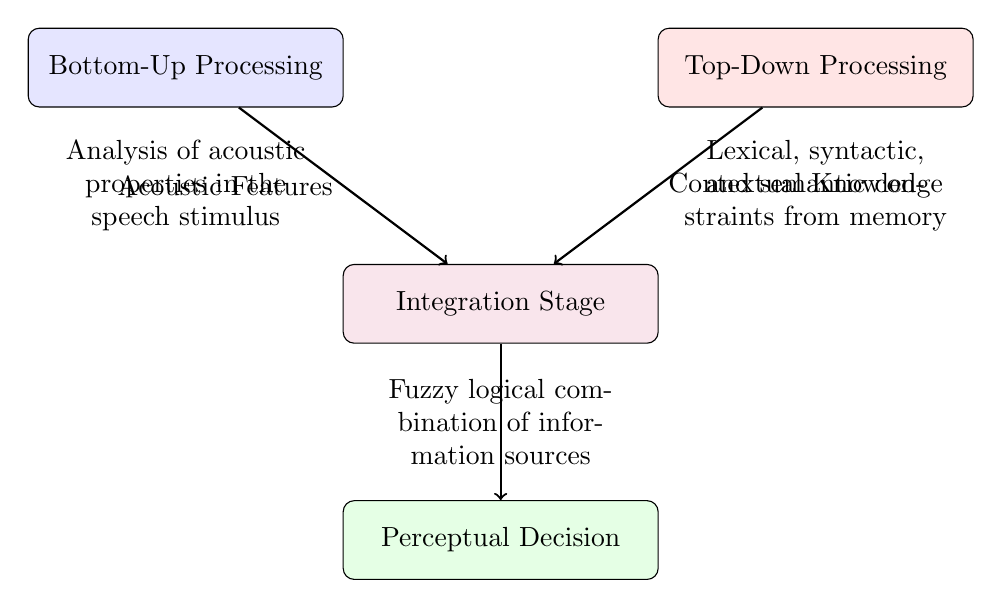
\begin{tikzpicture}[node distance=2.5cm]
    \node[draw, rectangle, rounded corners, fill=blue!10, minimum width=4cm, minimum height=1cm] (bottomup) at (0,0) {Bottom-Up Processing};
    \node[draw, rectangle, rounded corners, fill=red!10, minimum width=4cm, minimum height=1cm] (topdown) at (8,0) {Top-Down Processing};
    
    \node[draw, rectangle, rounded corners, fill=purple!10, minimum width=4cm, minimum height=1cm] (integration) at (4,-3) {Integration Stage};
    \node[draw, rectangle, rounded corners, fill=green!10, minimum width=4cm, minimum height=1cm] (percept) at (4,-6) {Perceptual Decision};
    
    \draw[->, thick] (bottomup) -- node[left] {Acoustic Features} (integration);
    \draw[->, thick] (topdown) -- node[right] {Contextual Knowledge} (integration);
    \draw[->, thick] (integration) -- (percept);
    
    \node[text width=3.5cm, align=center] at (0,-1.5) {Analysis of acoustic properties in the speech stimulus};
    \node[text width=3.5cm, align=center] at (8,-1.5) {Lexical, syntactic, and semantic constraints from memory};
    
    \node[text width=3.5cm, align=center] at (4,-4.5) {Fuzzy logical combination of information sources};
\end{tikzpicture}
\caption{The Fuzzy Logic Model of Perception (FLMP) framework}
\label{fig:flmp_framework}
\end{figure}

This model has historical precedent in philosophical discussions of perception. Immanuel Kant distinguished between sensory impressions and the categories of understanding that shape our experience—a distinction that parallels the bottom-up/top-down division in FLMP. Similarly, the Gestalt psychologists argued that our perceptions emerge from the interaction between sensory data and organizational principles of the mind.

\begin{tcolorbox}[title=Historical Perspective: From Philosophy to Cognitive Science]
The integration of bottom-up and top-down processes central to FLMP reflects philosophical debates dating back centuries. The British Empiricists (Locke, Berkeley, Hume) emphasized that knowledge comes primarily through sensory experience (analogous to bottom-up processing), while Rationalists like Descartes and Leibniz argued that certain knowledge structures are innate or constructed by the mind (analogous to top-down processing).

The modern cognitive revolution of the 1950s synthesized these perspectives, recognizing that perception involves both sensory data and interpretative frameworks—a perspective formalized in FLMP's mathematical framework for speech perception.
\end{tcolorbox}

\subsection{Prototype Matching and Fuzzy Logic}

The FLMP proposes that phonemes are represented as acoustic prototypes in long-term memory. These prototypes specify the ideal acoustic features associated with each phoneme. When we hear speech, the bottom-up processes extract acoustic features from the signal and compare them to these stored prototypes.

Crucially, this matching process operates according to principles of fuzzy logic rather than binary logic. In fuzzy logic, category membership is a matter of degree rather than an all-or-nothing affair. A sound might activate the /b/ phoneme prototype to a value of 0.7 and the /p/ phoneme prototype to a value of 0.3.

\begin{figure}[h]
\centering
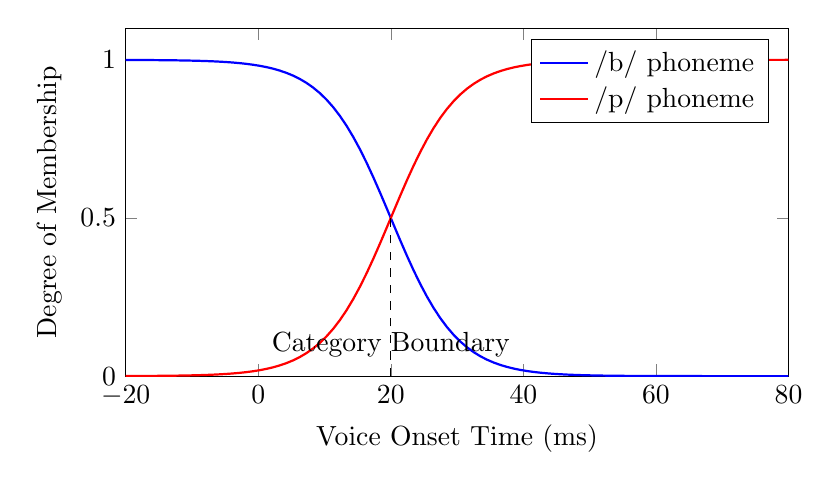
\begin{tikzpicture}
    \begin{axis}[
        width=10cm,
        height=6cm,
        xlabel=Voice Onset Time (ms),
        ylabel=Degree of Membership,
        xmin=-20, xmax=80,
        ymin=0, ymax=1.1,
        legend pos=north east,
        domain=-20:80,
        samples=100,
    ]
    
    \addplot[color=blue, thick] {1/(1+exp((x-20)/5))};
    \addlegendentry{/b/ phoneme}
    
    \addplot[color=red, thick] {1/(1+exp(-(x-20)/5))};
    \addlegendentry{/p/ phoneme}
    
    \draw[dashed] (axis cs:20,0) -- (axis cs:20,0.5);
    \node at (axis cs:20,0.1) {Category Boundary};
    
    \end{axis}
\end{tikzpicture}
\caption{Fuzzy membership functions for /b/ and /p/ phonemes based on Voice Onset Time}
\label{fig:fuzzy_membership}
\end{figure}

This fuzzy logic approach elegantly explains categorical perception—the tendency to perceive speech sounds as belonging to discrete categories despite continuous variation in the acoustic signal. The sigmoid shapes of the membership functions in Figure \ref{fig:fuzzy_membership} explain why listeners are more sensitive to acoustic differences that cross category boundaries than to equally large acoustic differences within a category.

\subsection{The Ganong Effect: Lexical Knowledge Shapes Perception}

One of the most compelling demonstrations of top-down influence in speech perception is the Ganong Effect, named after William Ganong who first documented it in 1980. This effect reveals how our knowledge of words biases phoneme perception.

\begin{tcolorbox}[enhanced, colback=yellow!5, colframe=yellow!75!black, title=The Ganong Effect Demonstrated]

Consider these two conditions:

\begin{center}
\begin{tabular}{|c|c|}
\hline
\textbf{Ambiguous Sound} & \textbf{Context} \\
\hline
Midway between /d/ and /t/ & "\_ash" (could be "dash" or "tash") \\
\hline
Midway between /d/ and /t/ & "\_ask" (could be "dask" or "task") \\
\hline
\end{tabular}
\end{center}

Listeners typically hear "dash" in the first condition (because "tash" is not a word) and "task" in the second condition (because "dask" is not a word). The identical ambiguous sound is interpreted differently based on which interpretation creates a real word.
\end{tcolorbox}

The philosopher John Dewey anticipated such effects in his pragmatic theory of perception, arguing that perception is shaped by our practical needs and expectations. Similarly, the Ganong Effect demonstrates that speech perception is not merely a matter of analyzing acoustic signals but involves integrating that analysis with our linguistic knowledge to reach the most probable interpretation.

\section{Phonemic Restoration: The Mind Filling the Gaps}

Perhaps the most dramatic demonstration of top-down influence in speech perception is the phonemic restoration effect, where listeners perceive phonemes that have been physically removed from the speech signal and replaced with noise.

\subsection{The Illusion of Continuity}

In a classic experiment by Richard Warren (1970), participants listened to recordings where a phoneme was replaced by a cough—for example, "The state governors met with their legi\textit{*cough*}lators." Remarkably, listeners not only failed to notice the missing phoneme but could not accurately locate where in the word the cough had occurred.

\begin{figure}[h]
\centering
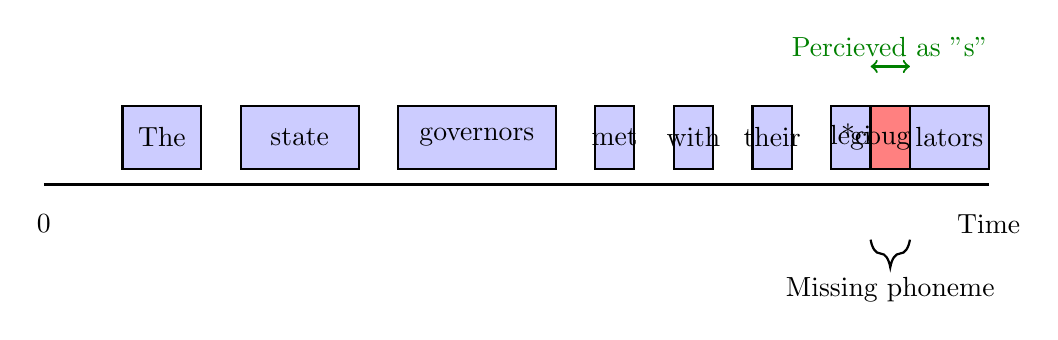
\begin{tikzpicture}
    \draw[thick] (0,0) -- (12,0);
    \node at (0,-0.5) {0};
    \node at (12,-0.5) {Time};
    
    \draw[thick, fill=blue!20] (1,0.2) rectangle (2,1) node[midway] {The};
    \draw[thick, fill=blue!20] (2.5,0.2) rectangle (4,1) node[midway] {state};
    \draw[thick, fill=blue!20] (4.5,0.2) rectangle (6.5,1) node[midway] {governors};
    \draw[thick, fill=blue!20] (7,0.2) rectangle (7.5,1) node[midway] {met};
    \draw[thick, fill=blue!20] (8,0.2) rectangle (8.5,1) node[midway] {with};
    \draw[thick, fill=blue!20] (9,0.2) rectangle (9.5,1) node[midway] {their};
    \draw[thick, fill=blue!20] (10,0.2) rectangle (10.5,1) node[midway] {legi};
    \draw[thick, fill=red!50] (10.5,0.2) rectangle (11,1) node[midway] {*cough*};
    \draw[thick, fill=blue!20] (11,0.2) rectangle (12,1) node[midway] {lators};
    
    \draw[thick, decorate, decoration={brace, amplitude=10pt, mirror}] (10.5,-0.7) -- (11,-0.7) node[midway, below, yshift=-10pt] {Missing phoneme};
    
    \draw[<->, thick, color=green!50!black] (10.5,1.5) -- (11,1.5) node[midway, above] {Percieved as "s"};
\end{tikzpicture}
\caption{Illustration of the phonemic restoration effect}
\label{fig:phonemic_restoration}
\end{figure}

This remarkable illusion demonstrates the brain's ability to reconstruct coherent percepts from incomplete sensory information. The process resembles the Bayesian inference methods increasingly popular in artificial intelligence—the brain generates the most probable interpretation given both the available sensory data and prior knowledge.

\subsection{Contextual Influences on Restoration}

The specific phoneme that listeners "restore" depends on the surrounding linguistic context. Samuel (1981) demonstrated this with ambiguous contexts:

\begin{tcolorbox}[enhanced, colback=green!5, colframe=green!75!black, title=Context-Dependent Restoration]
When listeners hear:
\begin{itemize}
\item "The wagon lost its \textit{*noise*}eel."
\item "The circus has a trained \textit{*noise*}eel."
\end{itemize}

In the first sentence, they typically restore a /w/, hearing "wheel."\\
In the second sentence, they typically restore an /s/, hearing "seal."
\end{tcolorbox}

Neuroscience research using event-related potentials (ERPs) reveals that the brain actually registers the noise about 200ms after it appears in the stimulus, but higher-level processes then incorporate this noise into a coherent linguistic interpretation. This finding connects to philosopher Maurice Merleau-Ponty's phenomenological view that perception involves active construction rather than passive reception.

\begin{figure}[h]
\centering
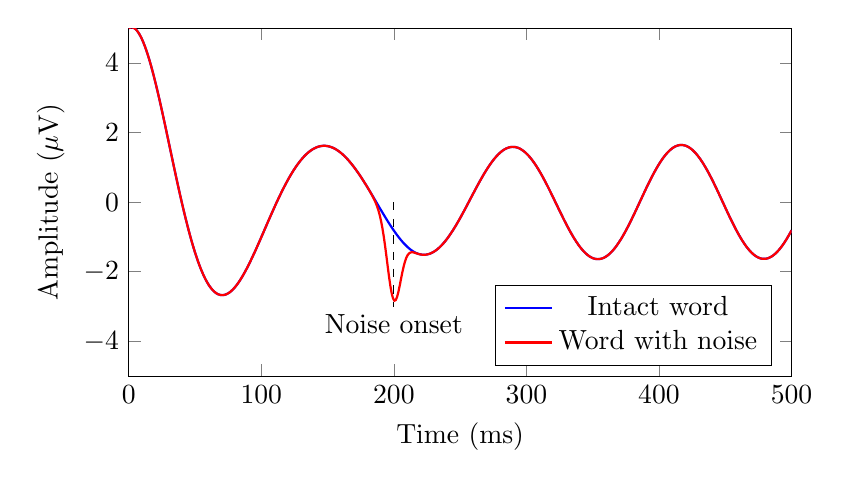
\begin{tikzpicture}
    \begin{axis}[
        width=10cm,
        height=6cm,
        xlabel=Time (ms),
        ylabel=Amplitude ($\mu$V),
        xmin=0, xmax=500,
        ymin=-5, ymax=5,
        legend pos=south east,
        domain=0:500,
        samples=500,
    ]
    
    \addplot[color=blue, thick] {1.5*sin(deg(0.05*x)) - 0.5*exp(-0.005*x)*(x-200)*0.05*cos(deg(0.05*x))};
    \addlegendentry{Intact word}
    
    \addplot[color=red, thick] {1.5*sin(deg(0.05*x)) - 2*exp(-0.02*(x-200)^2) - 0.5*exp(-0.005*x)*(x-200)*0.05*cos(deg(0.05*x))};
    \addlegendentry{Word with noise}
    
    \draw[dashed] (axis cs:200,0) -- (axis cs:200,-3);
    \node at (axis cs:200,-3.5) {Noise onset};
    
    \end{axis}
\end{tikzpicture}
\caption{Simulated ERP responses to intact words versus words with noise replacement}
\label{fig:erp_phonemic}
\end{figure}

\subsection{Theoretical Implications of Restoration Effects}

Phonemic restoration effects have profound implications for theories of speech perception. They challenge purely bottom-up models by demonstrating that perception incorporates prior knowledge and expectations. However, they also present challenges for motor theories, since listeners can "restore" phonemes they have physically never heard in that context.

The FLMP explains restoration effects through its integration mechanism. When a phoneme is replaced by noise, bottom-up processes extract whatever acoustic features remain. Top-down processes, operating simultaneously, activate phoneme prototypes consistent with lexical, syntactic, and semantic constraints. The integration stage combines these sources, with top-down information compensating for the missing bottom-up information.

\begin{figure}[h]
\centering
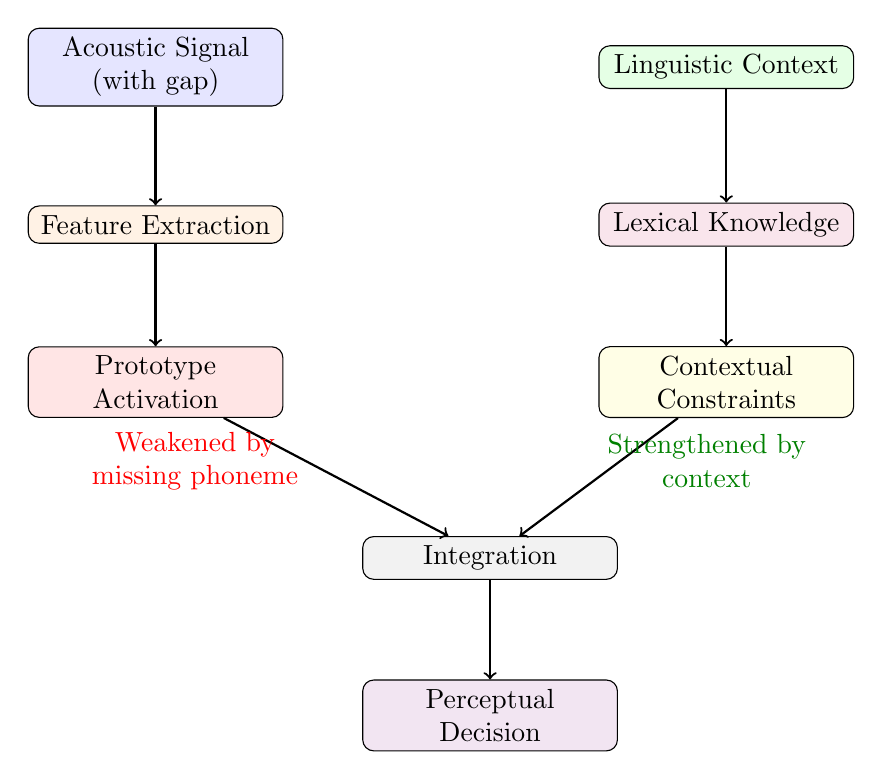
\begin{tikzpicture}[node distance=2cm, auto]
    \node[draw, rectangle, rounded corners, fill=blue!10, text width=3cm, align=center] (acoustic) {Acoustic Signal\\(with gap)};
    \node[draw, rectangle, rounded corners, fill=orange!10, text width=3cm, align=center, below of=acoustic] (extraction) {Feature Extraction};
    \node[draw, rectangle, rounded corners, fill=red!10, text width=3cm, align=center, below of=extraction] (prototype) {Prototype Activation};
    
    \node[draw, rectangle, rounded corners, fill=green!10, text width=3cm, align=center, right=4cm of acoustic] (context) {Linguistic Context};
    \node[draw, rectangle, rounded corners, fill=purple!10, text width=3cm, align=center, below of=context] (lexical) {Lexical Knowledge};
    \node[draw, rectangle, rounded corners, fill=yellow!10, text width=3cm, align=center, below of=lexical] (constraints) {Contextual Constraints};
    
    \node[draw, rectangle, rounded corners, fill=gray!10, text width=3cm, align=center, below right=1.5cm and 1cm of prototype] (integration) {Integration};
    
    \node[draw, rectangle, rounded corners, fill=violet!10, text width=3cm, align=center, below of=integration] (percept) {Perceptual Decision};
    
    \draw[->, thick] (acoustic) -- (extraction);
    \draw[->, thick] (extraction) -- (prototype);
    \draw[->, thick] (prototype) -- (integration);
    
    \draw[->, thick] (context) -- (lexical);
    \draw[->, thick] (lexical) -- (constraints);
    \draw[->, thick] (constraints) -- (integration);
    
    \draw[->, thick] (integration) -- (percept);
    
    \node[text width=3cm, align=center, red] at (0.5,-5) {Weakened by\\missing phoneme};
    \node[text width=3cm, align=center, green!50!black] at (7,-5) {Strengthened by\\context};
\end{tikzpicture}
\caption{How the FLMP accounts for phonemic restoration}
\label{fig:flmp_restoration}
\end{figure}

\section{Connectionist Models: Learning the Patterns of Speech}

The 1980s witnessed the emergence of connectionist or neural network models of speech perception. These models represent a paradigm shift from rule-based approaches toward systems that learn statistical regularities from experience with speech.

\subsection{From Symbolic Rules to Statistical Learning}

Traditional speech perception theories relied heavily on symbolic representations and explicit rules. Connectionist models, in contrast, emphasize how statistical learning can extract regularities from speech without explicit representations of rules or prototypes.

\begin{figure}[h]
\centering
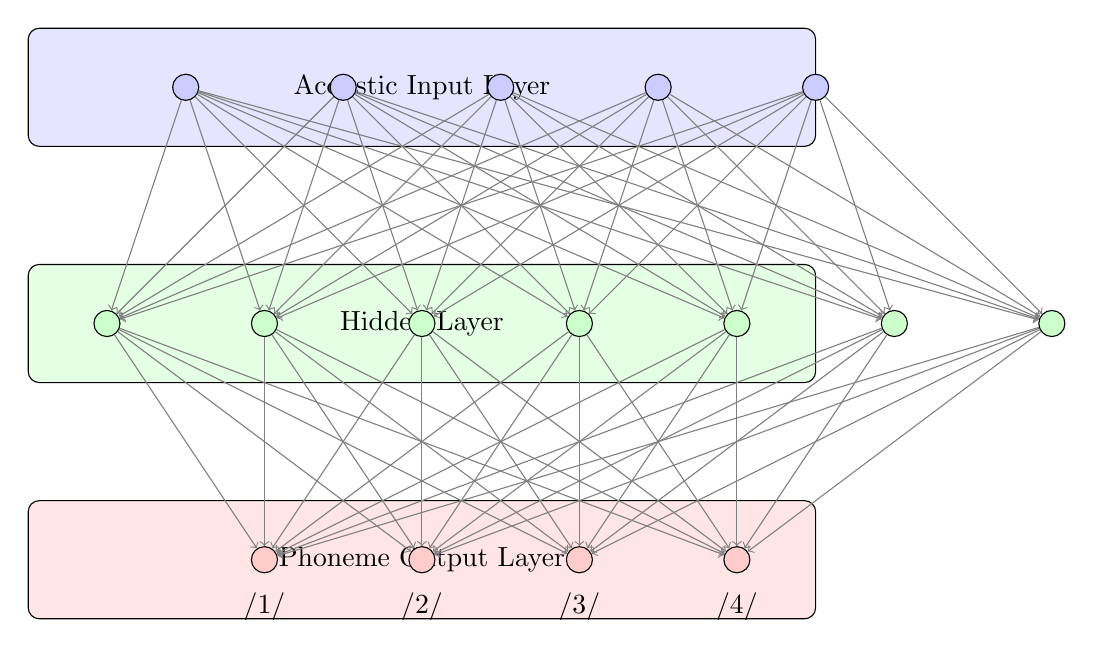
\begin{tikzpicture}
    \node[draw, rectangle, rounded corners, fill=blue!10, minimum width=10cm, minimum height=1.5cm] (input) at (0,0) {Acoustic Input Layer};
    
    \node[draw, rectangle, rounded corners, fill=green!10, minimum width=10cm, minimum height=1.5cm] (hidden) at (0,-3) {Hidden Layer};
    
    \node[draw, rectangle, rounded corners, fill=red!10, minimum width=10cm, minimum height=1.5cm] (output) at (0,-6) {Phoneme Output Layer};
    
    \foreach \i in {1,...,5} {
        \node[circle, draw, fill=blue!20] (in\i) at (-5+2*\i, 0) {};
    }
    
    \foreach \i in {1,...,7} {
        \node[circle, draw, fill=green!20] (hid\i) at (-6+2*\i, -3) {};
    }
    
    \foreach \i in {1,...,4} {
        \node[circle, draw, fill=red!20] (out\i) at (-4+2*\i, -6) {};
        \node[below=0.3cm] at (out\i) {/\i/};
    }
    
    \foreach \i in {1,...,5} {
        \foreach \j in {1,...,7} {
            \draw[->, thin, gray] (in\i) -- (hid\j);
        }
    }
    
    \foreach \i in {1,...,7} {
        \foreach \j in {1,...,4} {
            \draw[->, thin, gray] (hid\i) -- (out\j);
        }
    }
\end{tikzpicture}
\caption{A simple connectionist network for speech perception}
\label{fig:connectionist_network}
\end{figure}

This shift in modeling perspective parallels historical transitions in other sciences. Just as Darwin's theory of natural selection replaced the notion of divinely designed species with a process of statistical adaptation over time, connectionist models replace the notion of innate phonological rules with statistical learning processes.

The philosopher John Stuart Mill anticipated aspects of connectionist thinking in his theory of associationism, arguing that complex mental phenomena emerge from the association of simpler elements—much as connectionist networks learn complex patterns through associations between simple processing units.

\subsection{TRACE: A Landmark Connectionist Model}

The TRACE model, developed by James McClelland and Jeffrey Elman in 1986, represents a landmark connectionist approach to speech perception. Unlike FLMP, which focuses on the integration of distinct processing streams, TRACE emphasizes the role of activation and competition within a dynamic, interactive network.

\begin{tcolorbox}[enhanced, colback=purple!5, colframe=purple!75!black, title=The TRACE Architecture]
TRACE consists of three interconnected levels of processing units:

\begin{enumerate}
\item \textbf{Feature Level} - Units represent acoustic features like voicing, frication, and nasality
\item \textbf{Phoneme Level} - Units represent individual phonemes (/b/, /a/, /t/, etc.)
\item \textbf{Word Level} - Units represent entire words ("bat," "cat," "hat," etc.)
\end{enumerate}

Units within each level compete with each other through lateral inhibition, while units between adjacent levels activate each other through excitatory connections. This architecture allows information to flow both bottom-up (features → phonemes → words) and top-down (words → phonemes).
\end{tcolorbox}
\subsection{The Temporal Dimension in TRACE: Processing Speech Over Time}

TRACE derives its name from its ability to create a "trace" of activation patterns over time, preserving information about the temporal structure of speech. This temporal dimension is crucial for speech perception, as the same acoustic feature may be interpreted differently depending on its position in the speech stream and surrounding context.

Unlike simpler models that process all input simultaneously, TRACE replicates its entire network structure repeatedly along a temporal dimension—creating multiple copies of feature, phoneme, and word detectors at different time slices. This allows the model to capture the inherently sequential nature of speech.

\begin{tcolorbox}[enhanced, colback=yellow!5, colframe=yellow!75!black, title=TRACE's Temporal Dimension]
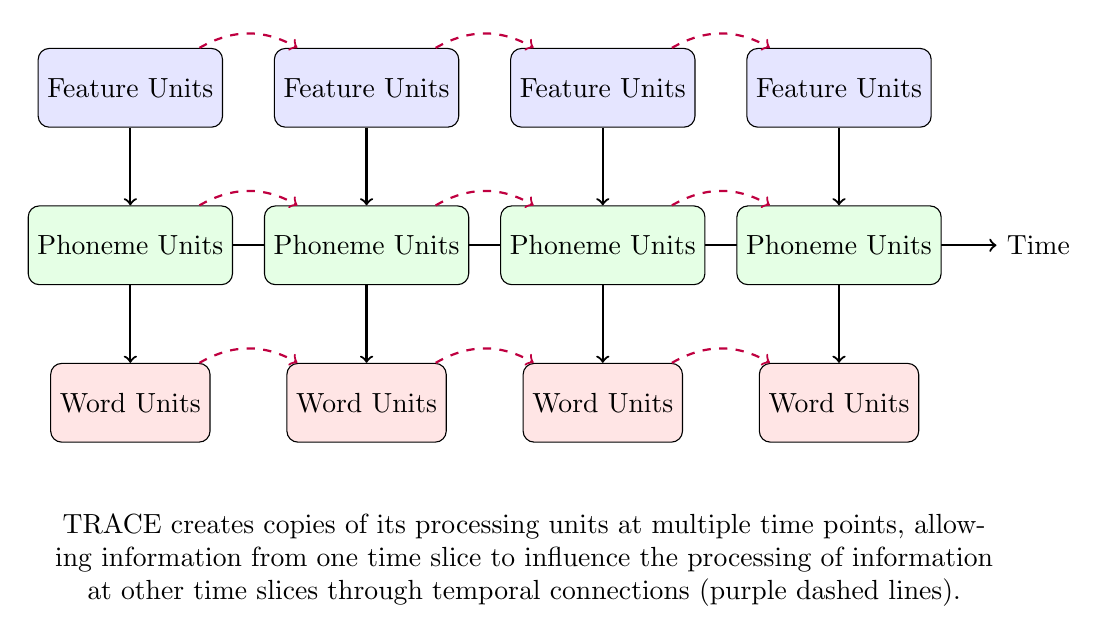
\begin{tikzpicture}
    \draw[thick, ->] (0,0) -- (12,0) node[right] {Time};
    
    \foreach \x in {1,4,7,10} {
        \node[draw, rectangle, rounded corners, fill=blue!10, minimum width=2cm, minimum height=1cm] (feature\x) at (\x,2) {Feature Units};
        \node[draw, rectangle, rounded corners, fill=green!10, minimum width=2cm, minimum height=1cm] (phoneme\x) at (\x,0) {Phoneme Units};
        \node[draw, rectangle, rounded corners, fill=red!10, minimum width=2cm, minimum height=1cm] (word\x) at (\x,-2) {Word Units};
        
        \draw[->, thick] (feature\x) -- (phoneme\x);
        \draw[->, thick] (phoneme\x) -- (word\x);
    }
    
    \foreach \x/\y in {1/4,4/7,7/10} {
        \draw[->, thick, dashed, color=purple] (feature\x) to[bend left=30] (feature\y);
        \draw[->, thick, dashed, color=purple] (phoneme\x) to[bend left=30] (phoneme\y);
        \draw[->, thick, dashed, color=purple] (word\x) to[bend left=30] (word\y);
    }
    
    \node[text width=12cm, align=center] at (6,-4) {TRACE creates copies of its processing units at multiple time points, allowing information from one time slice to influence the processing of information at other time slices through temporal connections (purple dashed lines).};
\end{tikzpicture}
\end{tcolorbox}

\subsubsection{Historical Context: Time as the Fourth Dimension of Speech}

The importance of time in speech perception has been recognized since the early phoneticians of the late 19th century. Physicist Hermann von Helmholtz noted in his 1863 work \textit{On the Sensations of Tone} that "the ear is able to distinguish an enormous number of sounds... [and] is also able to discriminate the constituents of a composite sound," but that these discriminations occur through patterns unfolding over time.

William James later observed in his \textit{Principles of Psychology} (1890) that consciousness itself has a "stream-like" quality—an insight that foreshadowed modern understandings of speech perception as the processing of patterns in a temporal stream rather than discrete static events.

\subsubsection{Why Temporal Processing Matters: Context-Dependent Interpretation}

The same acoustic feature can have dramatically different interpretations depending on its position in the speech stream and the surrounding context. Consider these examples:

\begin{tcolorbox}[enhanced, colback=green!5, colframe=green!75!black, title=Context-Dependent Acoustic Features]
\begin{tabular}{|p{3.5cm}|p{3.5cm}|p{3.5cm}|}
\hline
\textbf{Acoustic Feature} & \textbf{Context A} & \textbf{Context B} \\
\hline
35ms voice onset time & Perceived as /p/ in "pea" & Perceived as /b/ in rapid speech \\
\hline
Third formant transition & Signals /d/ before /i/ & Signals /g/ before /u/ \\
\hline
Short silent gap & Perceived as geminate consonant in Italian & Perceived as word boundary in English \\
\hline
\end{tabular}
\end{tcolorbox}

This context-dependency creates a fundamental challenge for speech perception models: how can the system correctly interpret variable acoustic features that lack a one-to-one mapping to linguistic units? TRACE addresses this challenge through its temporal structure and interactive processing.

\begin{figure}[h]
\centering
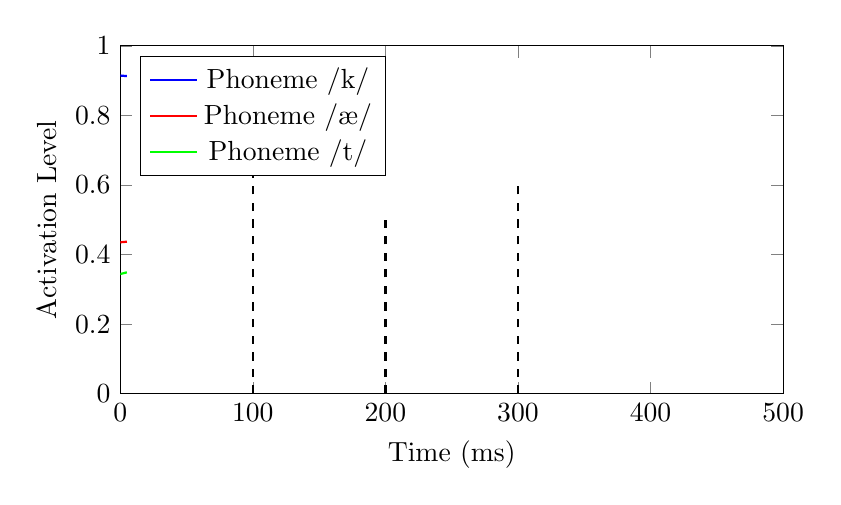
\begin{tikzpicture}
    \begin{axis}[
        width=10cm,
        height=6cm,
        xlabel=Time (ms),
        ylabel=Activation Level,
        xmin=0, xmax=500,
        ymin=0, ymax=1.0,
        legend pos=north west,
        samples=100,
    ]
    
    \addplot[color=blue, thick] {0.1*exp(-0.02*x) + 0.9*exp(-0.01*(x-100)^2/1000)};
    \addlegendentry{Phoneme /k/}
    
    \addplot[color=red, thick] {0.1*exp(-0.01*x) + 0.5*exp(-0.01*(x-200)^2/1000)};
    \addlegendentry{Phoneme /æ/}
    
    \addplot[color=green, thick] {0.1*exp(-0.005*x) + 0.6*exp(-0.01*(x-300)^2/1000)};
    \addlegendentry{Phoneme /t/}
    
    \draw[thick, dashed] (axis cs:100,0) -- (axis cs:100,0.9);
    \draw[thick, dashed] (axis cs:200,0) -- (axis cs:200,0.5);
    \draw[thick, dashed] (axis cs:300,0) -- (axis cs:300,0.6);
    
    \end{axis}
\end{tikzpicture}
\caption{Activation patterns of phonemes over time as TRACE processes the word "cat"}
\label{fig:trace_activation}
\end{figure}

\subsubsection{How TRACE Handles Time: The Reduplicated Network}

TRACE solves the temporal challenge through a unique architectural feature: reduplication of the entire network along a temporal dimension. Instead of trying to process an entire utterance at once, TRACE creates a series of processing units assigned to different time slices. Each time slice contains a complete copy of all feature, phoneme, and word detectors.

\begin{tcolorbox}[enhanced, colback=blue!5, colframe=blue!75!black, title=The Reduplicated Network Architecture]
\begin{center}
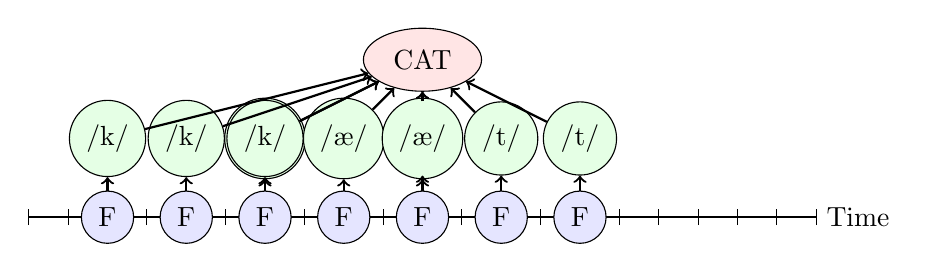
\begin{tikzpicture}
    \draw[thick] (0,0) -- (10,0) node[right] {Time};
    \foreach \x in {0,0.5,...,10} {
        \draw[thin] (\x,-0.1) -- (\x,0.1);
    }
    
    \node[draw, ellipse, fill=red!10, minimum width=1.5cm, minimum height=0.8cm] (cat) at (5,2) {CAT};
    
    \node[draw, circle, fill=green!10] (k1) at (1,1) {/k/};
    \node[draw, circle, fill=green!10] (a1) at (3,1) {/æ/};
    \node[draw, circle, fill=green!10] (t1) at (5,1) {/t/};
    
    \node[draw, circle, fill=green!10] (k2) at (2,1) {/k/};
    \node[draw, circle, fill=green!10] (a2) at (4,1) {/æ/};
    \node[draw, circle, fill=green!10] (t2) at (6,1) {/t/};
    
    \node[draw, circle, fill=green!10] (k3) at (3,1) {/k/};
    \node[draw, circle, fill=green!10] (a3) at (5,1) {/æ/};
    \node[draw, circle, fill=green!10] (t3) at (7,1) {/t/};
    
    \draw[->, thick] (k1) -- (cat);
    \draw[->, thick] (a1) -- (cat);
    \draw[->, thick] (t1) -- (cat);
    
    \draw[->, thick] (k2) -- (cat);
    \draw[->, thick] (a2) -- (cat);
    \draw[->, thick] (t2) -- (cat);
    
    \draw[->, thick] (k3) -- (cat);
    \draw[->, thick] (a3) -- (cat);
    \draw[->, thick] (t3) -- (cat);
    
    \node[draw, circle, fill=blue!10] (f1) at (1,0) {F};
    \node[draw, circle, fill=blue!10] (f2) at (2,0) {F};
    \node[draw, circle, fill=blue!10] (f3) at (3,0) {F};
    \node[draw, circle, fill=blue!10] (f4) at (4,0) {F};
    \node[draw, circle, fill=blue!10] (f5) at (5,0) {F};
    \node[draw, circle, fill=blue!10] (f6) at (6,0) {F};
    \node[draw, circle, fill=blue!10] (f7) at (7,0) {F};
    
    \draw[->, thick] (f1) -- (k1);
    \draw[->, thick] (f2) -- (k2);
    \draw[->, thick] (f3) -- (k3);
    \draw[->, thick] (f3) -- (a1);
    \draw[->, thick] (f4) -- (a2);
    \draw[->, thick] (f5) -- (a3);
    \draw[->, thick] (f5) -- (t1);
    \draw[->, thick] (f6) -- (t2);
    \draw[->, thick] (f7) -- (t3);
\end{tikzpicture}
\end{center}
\small Feature detectors (F) at different time points activate phoneme detectors (/k/, /æ/, /t/), which in turn activate word detectors (CAT). The same word can be recognized regardless of exactly when each phoneme is detected.
\end{tcolorbox}

This architecture allows TRACE to handle several key challenges in speech perception:

\begin{enumerate}
\item \textbf{Varying speech rates} - The same word can be recognized whether pronounced quickly or slowly
\item \textbf{Coarticulation effects} - Acoustic features modified by neighboring sounds can be correctly interpreted
\item \textbf{Segmentation} - Word boundaries can be identified without explicit markers
\item \textbf{Continuous recognition} - Processing begins as soon as acoustic information arrives, without waiting for an entire utterance
\end{enumerate}

\subsubsection{Philosophical Implications: Time and Perception}

TRACE's approach to temporal processing resonates with philosophical perspectives on time and perception. Henri Bergson's concept of "duration" (durée) proposed that consciousness experiences time not as a series of discrete moments but as a continuous flow where past, present, and future interpenetrate—similar to how TRACE integrates information across time slices.

Edmund Husserl's phenomenology similarly described consciousness as containing "retentions" (memories of just-past experiences) and "protentions" (anticipations of what will come next), creating a "specious present" that spans more than an instantaneous moment. This meshes well with TRACE's bidirectional flow of information across time slices.

\begin{tcolorbox}[enhanced, colback=purple!5, colframe=purple!75!black, title=The Philosophy of Time in Speech Perception]
\begin{center}
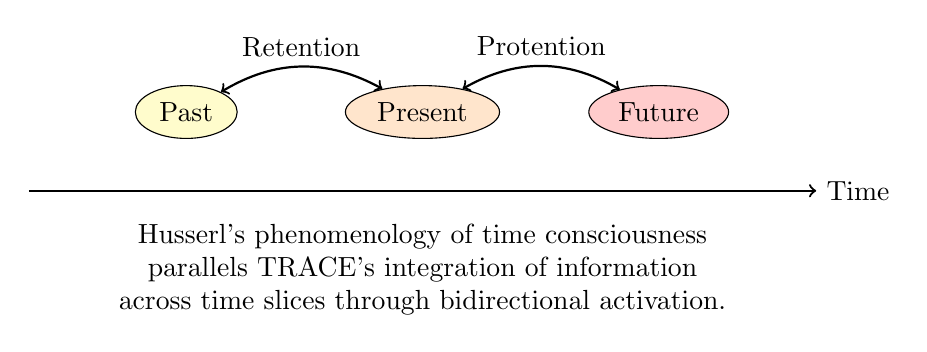
\begin{tikzpicture}
    \draw[thick, ->] (0,0) -- (10,0) node[right] {Time};
    
    \node[draw, ellipse, fill=yellow!20] (past) at (2,1) {Past};
    \node[draw, ellipse, fill=orange!20] (present) at (5,1) {Present};
    \node[draw, ellipse, fill=red!20] (future) at (8,1) {Future};
    
    \draw[<->, thick, bend left=30] (past) to node[above] {Retention} (present);
    \draw[<->, thick, bend left=30] (present) to node[above] {Protention} (future);
    
    \node[text width=8cm, align=center] at (5,-1) {Husserl's phenomenology of time consciousness parallels TRACE's integration of information across time slices through bidirectional activation.};
\end{tikzpicture}
\end{center}
\end{tcolorbox}

\subsubsection{Practical Applications: Speech Recognition Technology}

TRACE's innovations in handling temporal information have influenced modern speech recognition technologies. While early automatic speech recognition systems struggled with continuous speech, contemporary deep learning approaches incorporate similar principles to TRACE:

\begin{enumerate}
\item \textbf{Recurrent Neural Networks (RNNs)} explicitly model temporal dependencies through recurrent connections
\item \textbf{Long Short-Term Memory networks (LSTMs)} maintain information over extended time periods
\item \textbf{Attention mechanisms} dynamically focus on relevant parts of the input sequence, similar to TRACE's selective activation
\end{enumerate}

\begin{figure}[h]
\centering
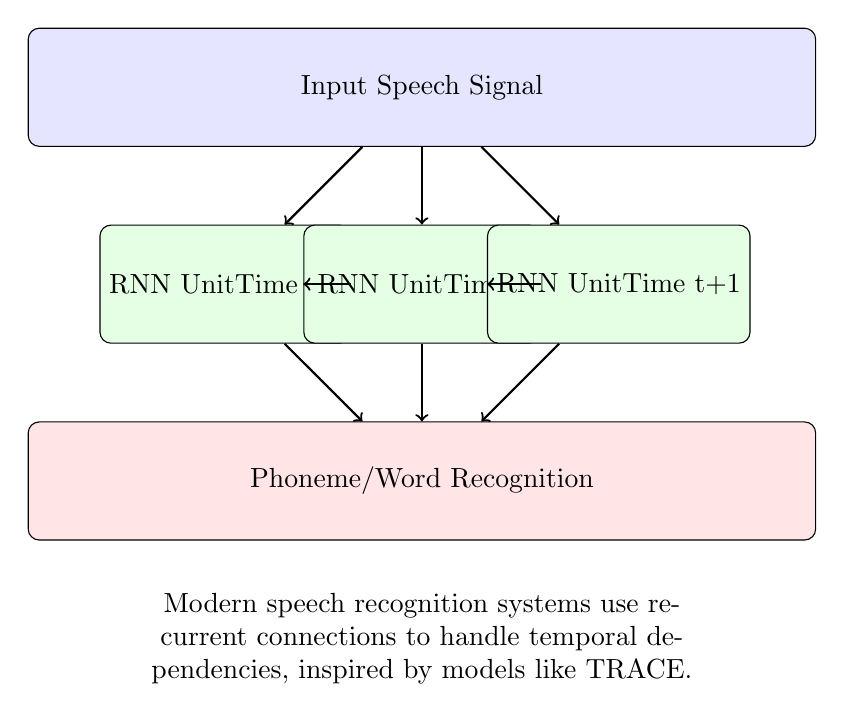
\begin{tikzpicture}
    \node[draw, rectangle, rounded corners, fill=blue!10, minimum width=10cm, minimum height=1.5cm] (input) at (0,0) {Input Speech Signal};
    
    \node[draw, rectangle, rounded corners, fill=green!10, minimum width=3cm, minimum height=1.5cm] (rnn1) at (-2.5,-2.5) {RNN Unit\\Time t-1};
    \node[draw, rectangle, rounded corners, fill=green!10, minimum width=3cm, minimum height=1.5cm] (rnn2) at (0,-2.5) {RNN Unit\\Time t};
    \node[draw, rectangle, rounded corners, fill=green!10, minimum width=3cm, minimum height=1.5cm] (rnn3) at (2.5,-2.5) {RNN Unit\\Time t+1};
    
    \node[draw, rectangle, rounded corners, fill=red!10, minimum width=10cm, minimum height=1.5cm] (output) at (0,-5) {Phoneme/Word Recognition};
    
    \draw[->, thick] (input) -- (rnn1);
    \draw[->, thick] (input) -- (rnn2);
    \draw[->, thick] (input) -- (rnn3);
    
    \draw[->, thick] (rnn1) -- (output);
    \draw[->, thick] (rnn2) -- (output);
    \draw[->, thick] (rnn3) -- (output);
    
    \draw[->, thick, bend left=30] (rnn1) -- (rnn2);
    \draw[->, thick, bend left=30] (rnn2) -- (rnn3);
    
    \node[text width=8cm, align=center] at (0,-7) {Modern speech recognition systems use recurrent connections to handle temporal dependencies, inspired by models like TRACE.};
\end{tikzpicture}
\caption{Recurrent neural networks for automatic speech recognition}
\label{fig:rnn_asr}
\end{figure}

\subsection{TRACE in Action: Simulating Perception Phenomena}

TRACE's power lies in its ability to simulate various phenomena in human speech perception. Let's explore some key examples that demonstrate how its temporal processing capabilities address real speech perception challenges.

\subsubsection{Lexical Effects on Phoneme Perception}

One of TRACE's most important contributions was demonstrating how higher-level lexical knowledge can influence lower-level phoneme perception—an interactive effect that emerges naturally from the model's bidirectional connections across time.

Consider the Ganong effect: When hearing an ambiguous sound between /d/ and /t/, listeners are more likely to perceive it as /d/ when followed by "ash" (creating "dash") but as /t/ when followed by "ask" (creating "task"). TRACE simulates this through feedback from the word level to the phoneme level.

\begin{tcolorbox}[enhanced, colback=orange!5, colframe=orange!75!black, title=TRACE Simulation of the Ganong Effect]
\begin{center}
\begin{tikzpicture}
    \node[draw, rectangle, rounded corners, fill=red!10, minimum width=3cm, minimum height=1cm] (dash) at (-2,2) {DASH};
    \node[draw, rectangle, rounded corners, fill=red!10, minimum width=3cm, minimum height=1cm] (tash) at (2,2) {TASH};
    
    \node[draw, rectangle, rounded corners, fill=green!10, minimum width=1.5cm, minimum height=1cm] (d) at (-3,0) {/d/};
    \node[draw, rectangle, rounded corners, fill=green!10, minimum width=1.5cm, minimum height=1cm] (t) at (-1,0) {/t/};
    \node[draw, rectangle, rounded corners, fill=green!10, minimum width=1.5cm, minimum height=1cm] (ash) at (0,0) {/æʃ/};
    
    \draw[->, thick] (d) -- (dash);
    \draw[->, thick] (t) -- (tash);
    \draw[->, thick] (ash) -- (dash);
    \draw[->, thick] (ash) -- (tash);
    
    \draw[->, thick, dashed, color=blue] (dash) to[bend right] (d);
    
    \node[text width=8cm, align=center] at (0,-2) {Since "dash" is a real word but "tash" is not, feedback from the word level boosts activation of /d/ when an ambiguous sound is heard.};
\end{tikzpicture}
\end{center}
\end{tcolorbox}

\subsubsection{Resolving Ambiguity Over Time}

Another strength of TRACE is its ability to resolve ambiguities as more information becomes available over time. For example, when hearing the beginning of "captain," the system initially activates words like "captain," "captive," and "capital." As more acoustic information arrives, the model narrows down the possibilities through competition and integration.

\begin{figure}[h]
\centering
\begin{tikzpicture}
    \begin{axis}[
        width=10cm,
        height=6cm,
        xlabel=Time (ms),
        ylabel=Word Activation,
        xmin=0, xmax=600,
        ymin=0, ymax=1.0,
        legend pos=north west,
        samples=100,
    ]
    
    \addplot[color=blue, thick] {0.2*exp(-0.002*x) + 0.8*exp(-0.01*(x-400)^2/40000)};
    \addlegendentry{CAPTAIN}
    
    \addplot[color=red, thick] {0.2*exp(-0.002*x) + 0.7*exp(-0.01*(x-300)^2/10000)};
    \addlegendentry{CAPTIVE}
    
    \addplot[color=green, thick] {0.2*exp(-0.002*x) + 0.5*exp(-0.01*(x-250)^2/8000)};
    \addlegendentry{CAPITAL}
    
    \draw[thick, dashed] (axis cs:100,0) -- (axis cs:100,0.8);
    \node at (axis cs:100,0.85) {/k/};
    
    \draw[thick, dashed] (axis cs:200,0) -- (axis cs:200,0.8);
    \node at (axis cs:200,0.85) {/æ/};
    
    \draw[thick, dashed] (axis cs:300,0) -- (axis cs:300,0.8);
    \node at (axis cs:300,0.85) {/p/};
    
    \draw[thick, dashed] (axis cs:400,0) -- (axis cs:400,0.8);
    \node at (axis cs:400,0.85) {/t/};
    
    \draw[thick, dashed] (axis cs:500,0) -- (axis cs:500,0.8);
    \node at (axis cs:500,0.85) {/ɪ/};
    
    \end{axis}
\end{tikzpicture}
\caption{TRACE activation patterns for competing words as acoustic information unfolds over time}
\label{fig:trace_competition}
\end{figure}

In this simulation, all three words are initially activated as the system processes /kæp/. As the input continues, "capital" begins losing activation when the /t/ is heard, followed by "captive" declining as /ɪ/ is processed. Finally, "captain" emerges as the winner as the complete acoustic information becomes available.

\subsubsection{Continuous Recognition and Segmentation}

Unlike many models that require pre-segmented input, TRACE can process continuous speech, identifying word boundaries through competition between lexical units. This capability emerges from its temporal structure and competitive inhibition.

Consider the phrase "recognize speech": Where does one word end and the next begin? TRACE addresses this through overlapping activation of word units at different time points, with the most consistent interpretations eventually winning out.

\begin{tcolorbox}[enhanced, colback=blue!5, colframe=blue!75!black, title=Segmentation Through Competition]
\begin{center}
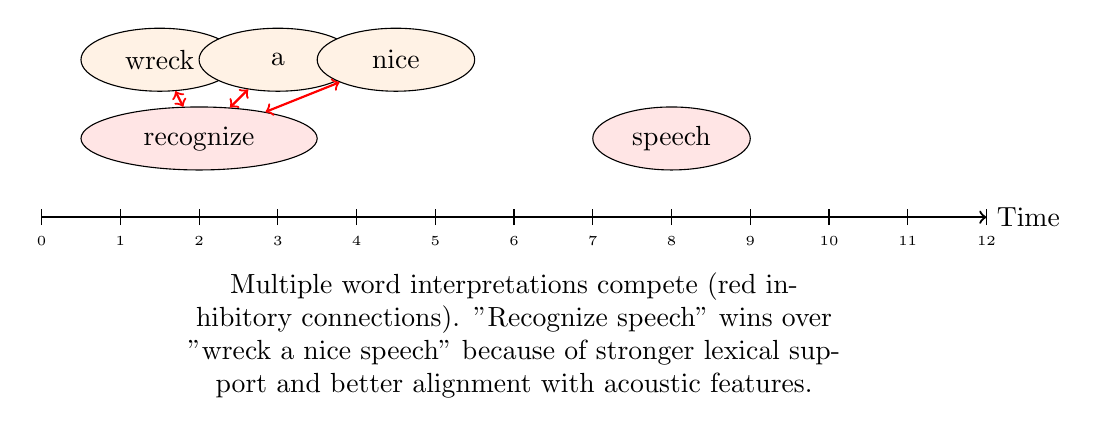
\begin{tikzpicture}
    \draw[thick, ->] (0,0) -- (12,0) node[right] {Time};
    \foreach \x in {0,1,...,12} {
        \draw[thin] (\x,-0.1) -- (\x,0.1);
        \node[font=\tiny] at (\x,-0.3) {\x};
    }
    
    \node[draw, ellipse, fill=red!10, minimum width=3cm, minimum height=0.8cm] (recog) at (2,1) {recognize};
    \node[draw, ellipse, fill=red!10, minimum width=2cm, minimum height=0.8cm] (speech) at (8,1) {speech};
    
    \node[draw, ellipse, fill=orange!10, minimum width=2cm, minimum height=0.8cm] (wreck) at (1.5,2) {wreck};
    \node[draw, ellipse, fill=orange!10, minimum width=2cm, minimum height=0.8cm] (a) at (3,2) {a};
    \node[draw, ellipse, fill=orange!10, minimum width=2cm, minimum height=0.8cm] (nice) at (4.5,2) {nice};
    
    \draw[<->, thick, red] (recog) -- (wreck);
    \draw[<->, thick, red] (recog) -- (a);
    \draw[<->, thick, red] (recog) -- (nice);
    
    \node[text width=10cm, align=center] at (6,-1.5) {Multiple word interpretations compete (red inhibitory connections). "Recognize speech" wins over "wreck a nice speech" because of stronger lexical support and better alignment with acoustic features.};
\end{tikzpicture}
\end{center}
\end{tcolorbox}

This emergent segmentation capability connects to the philosophical concept of "gestalt" from early 20th century psychology—the notion that perception involves organizing sensory elements into meaningful wholes based on principles like proximity, similarity, and continuity. TRACE demonstrates how word boundaries emerge naturally from the perceptual process rather than being explicitly marked in the signal.

\subsection{Extensions and Limitations of TRACE}

While TRACE has been remarkably successful in explaining many phenomena of speech perception, it has limitations that have inspired extensions and alternative models.

\subsubsection{Computational Complexity}

The reduplication of processing units across time makes TRACE computationally intensive. For every phoneme at every possible position, a separate unit is required, leading to a combinatorial explosion as utterance length increases.

\begin{tcolorbox}[enhanced, colback=red!5, colframe=red!75!black, title=TRACE's Computational Challenge]
\begin{center}
\begin{tabular}{|c|c|c|}
\hline
\textbf{Utterance Length} & \textbf{Number of Phoneme Units} & \textbf{Number of Word Units} \\
\hline
10 time slices & 400 (40 phonemes × 10 positions) & 2,000 (200 words × 10 positions) \\
\hline
50 time slices & 2,000 & 10,000 \\
\hline
100 time slices & 4,000 & 20,000 \\
\hline
\end{tabular}
\end{center}
\small This computational complexity has inspired more efficient models like PARSYN (Luce et al., 2000) that achieve similar functionality with recurrent connections rather than reduplicated units.
\end{tcolorbox}

\subsubsection{Learning and Development}

TRACE does not address how the network's connectivity is learned from experience. The model comes pre-equipped with connections, but doesn't explain how children acquire phonological categories or lexical representations.

Later models like TRACE II incorporated Hebbian learning mechanisms to address this limitation, allowing the network to modify connection weights based on co-occurrence statistics in the input.

\begin{figure}[h]
\centering
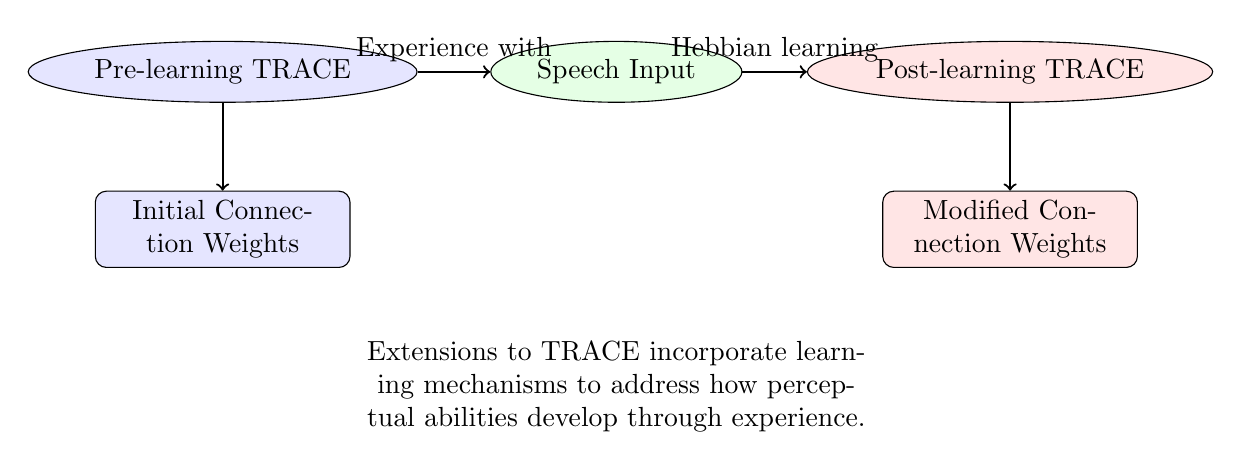
\begin{tikzpicture}
    \node[draw, ellipse, fill=blue!10] (prelearning) at (0,0) {Pre-learning TRACE};
    \node[draw, ellipse, fill=green!10] (input) at (5,0) {Speech Input};
    \node[draw, ellipse, fill=red!10] (postlearning) at (10,0) {Post-learning TRACE};
    
    \draw[->, thick] (prelearning) -- node[above] {Experience with} (input);
    \draw[->, thick] (input) -- node[above] {Hebbian learning} (postlearning);
    
    \node[draw, rectangle, rounded corners, fill=blue!10, text width=3cm, align=center] (preconn) at (0,-2) {Initial Connection Weights};
    \node[draw, rectangle, rounded corners, fill=red!10, text width=3cm, align=center] (postconn) at (10,-2) {Modified Connection Weights};
    
    \draw[->, thick] (prelearning) -- (preconn);
    \draw[->, thick] (postlearning) -- (postconn);
    
    \node[text width=8cm, align=center] at (5,-4) {Extensions to TRACE incorporate learning mechanisms to address how perceptual abilities develop through experience.};
\end{tikzpicture}
\caption{Incorporating learning mechanisms into TRACE}
\label{fig:trace_learning}
\end{figure}

\subsubsection{Lack of Episodic Representations}

TRACE operates with abstract, context-independent representations of phonemes and words. However, research suggests that humans retain episodic traces of specific instances of words, including speaker characteristics, emotional tone, and situational context.

\begin{tcolorbox}[enhanced, colback=green!5, colframe=green!75!black, title=Episodic vs. Abstract Representations]
\begin{tabular}{|p{4cm}|p{4cm}|p{4cm}|}
\hline
\textbf{Aspect} & \textbf{TRACE (Abstract)} & \textbf{Episodic Models} \\
\hline
Speaker variation & Treated as noise to be filtered out & Retained as part of word representation \\
\hline
Multiple pronunciations & Single canonical form & Multiple exemplars stored \\
\hline
Recognition mechanism & Activation of abstract unit & Similarity to stored exemplars \\
\hline
\end{tabular}
\end{tcolorbox}

Models like MINERVA (Hintzman, 1986) and more recent exemplar-based approaches address this limitation by storing multiple episodic traces of each word and computing recognition based on similarity to these traces.

\subsection{TRACE's Legacy: Bridging Production and Perception}

Despite its limitations, TRACE's integration of temporal processing has profoundly influenced both theoretical and applied work in speech perception. Its approach to handling time resonates with current theories that emphasize prediction and anticipation in perception.

The model also provides a natural bridge to theories of speech production. While TRACE focuses on perception, its interactive architecture shares principles with production models like Dell's Spreading Activation model, suggesting potential unification of production and perception frameworks.

\begin{tcolorbox}[enhanced, colback=purple!5, colframe=purple!75!black, title=TRACE's Influence on Contemporary Theories]
\begin{center}
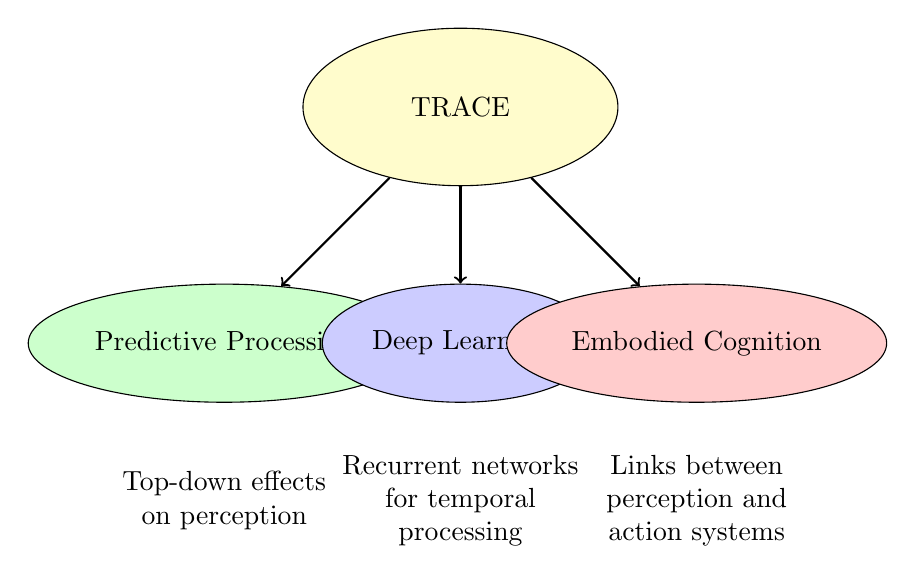
\begin{tikzpicture}
    \node[draw, ellipse, fill=yellow!20, minimum width=4cm, minimum height=2cm] (trace) at (0,0) {TRACE};
    
    \node[draw, ellipse, fill=green!20, minimum width=3cm, minimum height=1.5cm] (predictive) at (-3,-3) {Predictive Processing};
    \node[draw, ellipse, fill=blue!20, minimum width=3cm, minimum height=1.5cm] (deep) at (0,-3) {Deep Learning};
    \node[draw, ellipse, fill=red!20, minimum width=3cm, minimum height=1.5cm] (embodied) at (3,-3) {Embodied Cognition};
    
    \draw[->, thick] (trace) -- (predictive);
    \draw[->, thick] (trace) -- (deep);
    \draw[->, thick] (trace) -- (embodied);
    
    \node[text width=3cm, align=center] at (-3,-5) {Top-down effects on perception};
    \node[text width=3cm, align=center] at (0,-5) {Recurrent networks for temporal processing};
    \node[text width=3cm, align=center] at (3,-5) {Links between perception and action systems};
\end{tikzpicture}
\end{center}
\end{tcolorbox}

As philosopher Alva Noë noted, perception is not something that happens to us but something we do—an active process of exploration rather than passive reception. TRACE anticipated this view by modeling perception as an active, constructive process that unfolds over time rather than a simple bottom-up analysis of acoustic features.

From the specialized temporal processing of TRACE to the general communicative framework of the Shannon-Weaver model, our understanding of speech perception has evolved toward increasingly sophisticated accounts that recognize the dynamic, interactive nature of how we extract meaning from the speech signal.

\section{The Evolution of Speech Perception Models: From Specialized to Integrated Frameworks}

The progression from specialized temporal processing models like TRACE to broader communicative frameworks like Shannon-Weaver represents a fundamental shift in our understanding of speech perception. This evolution reflects how the field has moved from viewing speech perception as a specialized, modular process toward recognizing it as an integrated phenomenon that draws upon multiple sources of information and processing mechanisms.

\subsection{From Specialized Modules to Integrated Systems}

Early theories of speech perception, particularly Motor Theory, emphasized the special status of speech processing—proposing a dedicated module evolved specifically for analyzing speech signals. TRACE expanded this view by incorporating temporal processing and interactive activation but still focused primarily on phonological and lexical levels of speech processing.

\begin{tcolorbox}[enhanced, colback=blue!5, colframe=blue!75!black, title=The Evolution of Speech Perception Models]
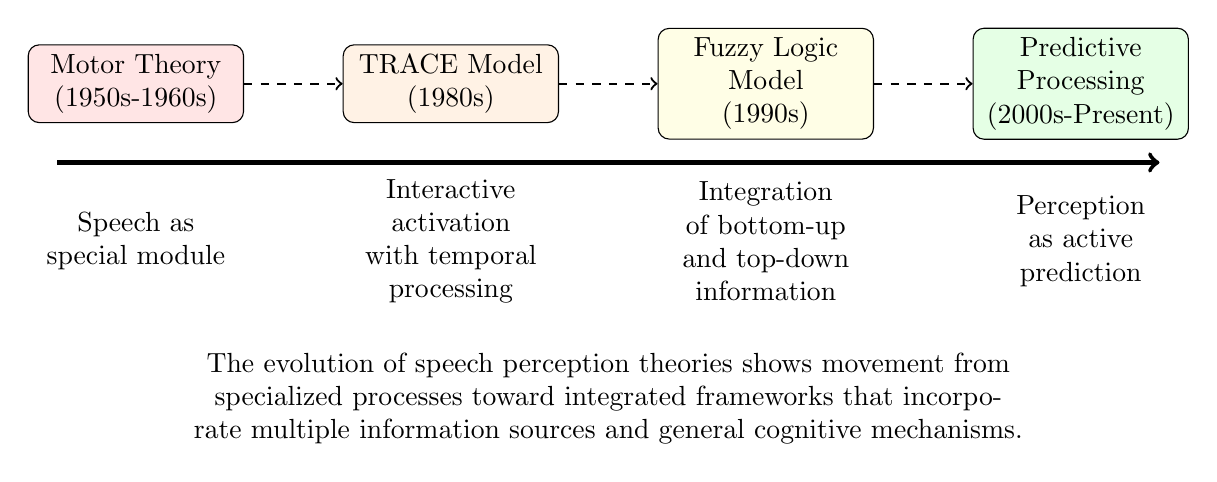
\begin{tikzpicture}
    \draw[->, ultra thick] (0,0) -- (14,0);
    
    \node[draw, rectangle, rounded corners, fill=red!10, text width=2.5cm, align=center] (motor) at (1,1) {Motor Theory\\(1950s-1960s)};
    \node[text width=2.5cm, align=center] at (1,-1) {Speech as special module};
    
    \node[draw, rectangle, rounded corners, fill=orange!10, text width=2.5cm, align=center] (trace) at (5,1) {TRACE Model\\(1980s)};
    \node[text width=2.5cm, align=center] at (5,-1) {Interactive activation with temporal processing};
    
    \node[draw, rectangle, rounded corners, fill=yellow!10, text width=2.5cm, align=center] (flmp) at (9,1) {Fuzzy Logic Model\\(1990s)};
    \node[text width=2.5cm, align=center] at (9,-1) {Integration of bottom-up and top-down information};
    
    \node[draw, rectangle, rounded corners, fill=green!10, text width=2.5cm, align=center] (predictive) at (13,1) {Predictive Processing\\(2000s-Present)};
    \node[text width=2.5cm, align=center] at (13,-1) {Perception as active prediction};
    
    \draw[->, thick, dashed] (motor) -- (trace);
    \draw[->, thick, dashed] (trace) -- (flmp);
    \draw[->, thick, dashed] (flmp) -- (predictive);
    
    \node[text width=12cm, align=center] at (7,-3) {The evolution of speech perception theories shows movement from specialized processes toward integrated frameworks that incorporate multiple information sources and general cognitive mechanisms.};
\end{tikzpicture}
\end{tcolorbox}

This evolution parallels broader shifts in cognitive science and artificial intelligence—from symbolic, rule-based approaches to statistical, learning-based approaches that emphasize the role of prediction and uncertainty in cognitive processing. The philosopher Daniel Dennett characterized this as a shift from viewing the mind as a "Cartesian Theater" with a central executive to seeing it as a "Pandemonium" of competing processes that collectively give rise to coherent experience.

\subsection{The Shannon-Weaver Model: Communication as Information Transfer}

The Shannon-Weaver model, developed in the late 1940s, offers a general framework for understanding communication processes, including speech perception. Unlike specialized speech perception theories, it focuses on the abstract problem of transferring information from one point to another, regardless of the specific medium or content.

\begin{figure}[h]
\centering
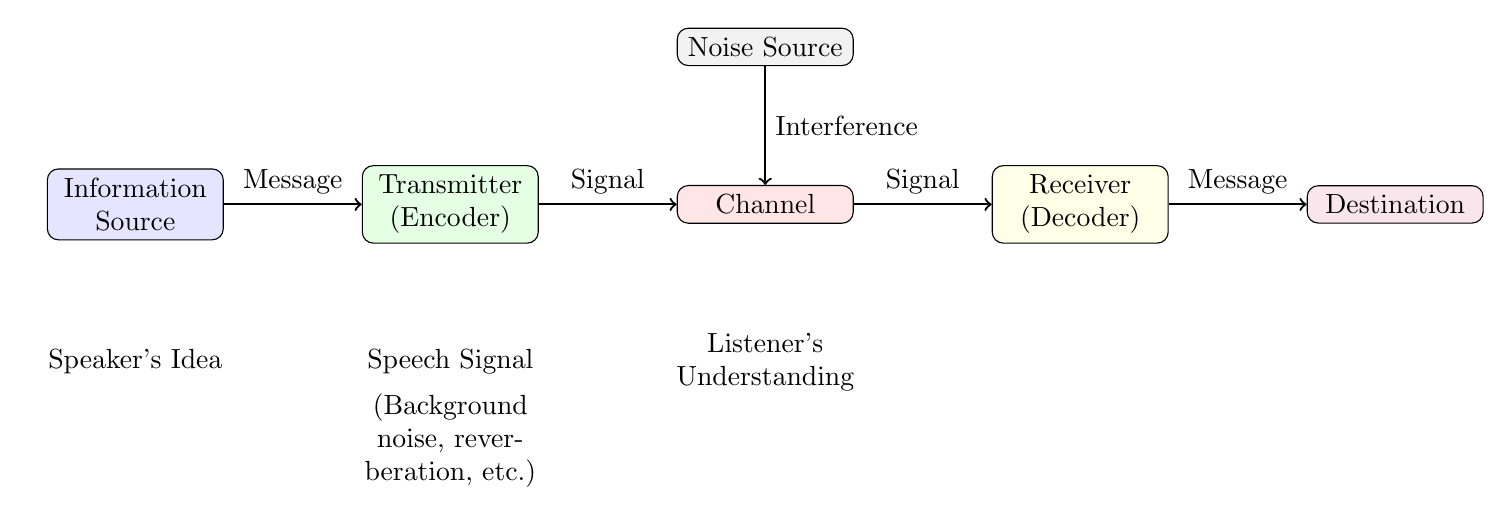
\begin{tikzpicture}[node distance=2cm, auto]
    \node[draw, rectangle, rounded corners, fill=blue!10, text width=2cm, align=center] (source) {Information Source};
    
    \node[draw, rectangle, rounded corners, fill=green!10, text width=2cm, align=center, right of=source, xshift=2cm] (transmitter) {Transmitter\\(Encoder)};
    
    \node[draw, rectangle, rounded corners, fill=red!10, text width=2cm, align=center, right of=transmitter, xshift=2cm] (channel) {Channel};
    
    \node[draw, rectangle, rounded corners, fill=yellow!10, text width=2cm, align=center, right of=channel, xshift=2cm] (receiver) {Receiver\\(Decoder)};
    
    \node[draw, rectangle, rounded corners, fill=purple!10, text width=2cm, align=center, right of=receiver, xshift=2cm] (destination) {Destination};
    
    \node[draw, rectangle, rounded corners, fill=gray!10, text width=2cm, align=center, above of=channel] (noise) {Noise Source};
    
    \draw[->, thick] (source) -- node[above] {Message} (transmitter);
    \draw[->, thick] (transmitter) -- node[above] {Signal} (channel);
    \draw[->, thick] (channel) -- node[above] {Signal} (receiver);
    \draw[->, thick] (receiver) -- node[above] {Message} (destination);
    \draw[->, thick] (noise) -- node[right] {Interference} (channel);
    
    \node[text width=2.5cm, align=center] at (0,-2) {Speaker's Idea};
    \node[text width=2.5cm, align=center] at (4,-2) {Speech Signal};
    \node[text width=2.5cm, align=center] at (8,-2) {Listener's\\Understanding};
    \node[text width=2.5cm, align=center] at (4,-3) {(Background noise, reverberation, etc.)};
\end{tikzpicture}
\caption{The Shannon-Weaver model applied to speech communication}
\label{fig:shannon_weaver}
\end{figure}

When applied to speech, the Shannon-Weaver model frames perception as a decoding problem: How does a listener recover the intended message from an acoustic signal that may be degraded by noise? This perspective highlights several important aspects of speech perception:

\begin{enumerate}
\item \textbf{Redundancy} - Human speech contains substantial redundancy, allowing messages to be reconstructed even when portions are missing or corrupted. This explains phenomena like phonemic restoration, where listeners "fill in" missing phonemes based on contextual information.

\item \textbf{Channel capacity} - There are limits to how much information can be transmitted through a given channel in a given time. This helps explain why speech perception sometimes fails in noisy environments or when speech rate increases beyond certain thresholds.

\item \textbf{Coding efficiency} - Languages evolve to balance communicative precision against the effort required for production and perception. Frequent words tend to be shorter, and phonological systems tend to maintain sufficient perceptual contrast between phonemes.
\end{enumerate}

\begin{tcolorbox}[enhanced, colback=green!5, colframe=green!75!black, title=Redundancy in Natural Languages]
\begin{center}
\begin{tabular}{|p{4cm}|p{8cm}|}
\hline
\textbf{Level of Redundancy} & \textbf{Examples in English} \\
\hline
Acoustic & Multiple acoustic cues signal the same phonemic contrast (e.g., VOT, F1 onset, and F2 transition all signal voicing) \\
\hline
Phonological & Constraints on possible sound combinations (e.g., English doesn't allow /bn/ at the beginning of words) \\
\hline
Lexical & Context constrains possible word identities (e.g., "The *eel of the car" must be "wheel") \\
\hline
Syntactic & Grammatical markers often appear multiple times (e.g., "Those tall boys are running" marks plurality four times) \\
\hline
\end{tabular}
\end{center}
\small Information theory quantifies this redundancy: English has approximately 75\% redundancy, meaning that accurate comprehension is possible even when significant portions of the signal are missing.
\end{tcolorbox}

While the Shannon-Weaver model provides valuable insights into general communication processes, it has significant limitations when applied to human speech perception:

\begin{table}[h]
\centering
\begin{tabular}{|p{5cm}|p{7cm}|}
\hline
\textbf{Limitation} & \textbf{Implication for Speech} \\
\hline
Linear, unidirectional flow & Speech perception involves continuous feedback between different levels of processing \\
\hline
Fixed, shared code assumption & Speech interpretation depends on social and contextual factors that vary across speakers and situations \\
\hline
Passive receiver model & Listeners actively construct meaning rather than simply decoding \\
\hline
Lack of intentionality & Human communication involves goals, intentions, and social motivations \\
\hline
\end{tabular}
\caption{Limitations of the Shannon-Weaver model for human speech perception}
\label{tbl:shannon_limitations}
\end{table}

These limitations have led to more sophisticated models that incorporate predictive processing, social cognition, and the active role of the listener in constructing meaning.

\subsection{Integrated Approaches: The Fuzzy Logic Model of Perception}

The Fuzzy Logic Model of Perception (FLMP) represents a significant step toward integrating multiple sources of information in speech perception. Developed by Dominic Massaro and colleagues, the FLMP proposes that speech perception emerges from the integration of bottom-up acoustic information and top-down knowledge.

\begin{figure}[h]
\centering
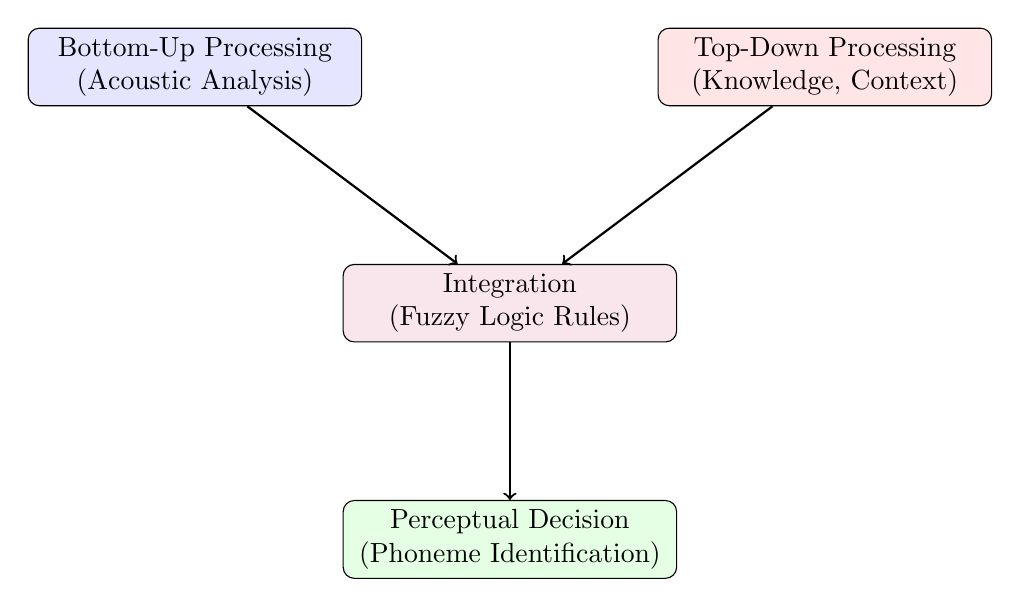
\begin{tikzpicture}
    \node[draw, rectangle, rounded corners, fill=blue!10, text width=4cm, align=center] (bottomup) at (0,0) {Bottom-Up Processing\\(Acoustic Analysis)};
    
    \node[draw, rectangle, rounded corners, fill=red!10, text width=4cm, align=center] (topdown) at (8,0) {Top-Down Processing\\(Knowledge, Context)};
    
    \node[draw, rectangle, rounded corners, fill=purple!10, text width=4cm, align=center] (integration) at (4,-3) {Integration\\(Fuzzy Logic Rules)};
    
    \node[draw, rectangle, rounded corners, fill=green!10, text width=4cm, align=center] (decision) at (4,-6) {Perceptual Decision\\(Phoneme Identification)};
    
    \draw[->, thick] (bottomup) -- (integration);
    \draw[->, thick] (topdown) -- (integration);
    \draw[->, thick] (integration) -- (decision);
\end{tikzpicture}
\caption{The Fuzzy Logic Model of Perception framework}
\label{fig:flmp_framework}
\end{figure}

The FLMP explains several key phenomena in speech perception:

\begin{enumerate}
\item \textbf{The Ganong Effect} - Ambiguous sounds tend to be perceived as creating real words. For example, an ambiguous sound between /d/ and /t/ is more likely to be perceived as /d/ when followed by "ash" (creating "dash") but as /t/ when followed by "ask" (creating "task").

\item \textbf{Phonemic Restoration} - When phonemes are replaced by noise (like a cough), listeners perceive the missing phoneme and often cannot even identify where the noise occurred. The specific phoneme "restored" depends on context: "The wagon lost its (cough)eel" is heard as "wheel," while "The circus has a trained (cough)eel" is heard as "seal."

\item \textbf{Multimodal Integration} - The model accounts for how visual information (as in the McGurk effect) and other sensory inputs are integrated with acoustic information.
\end{enumerate}

\begin{tcolorbox}[enhanced, colback=orange!5, colframe=orange!75!black, title=The Fuzzy Logic Approach to Multimodal Integration]
\begin{center}
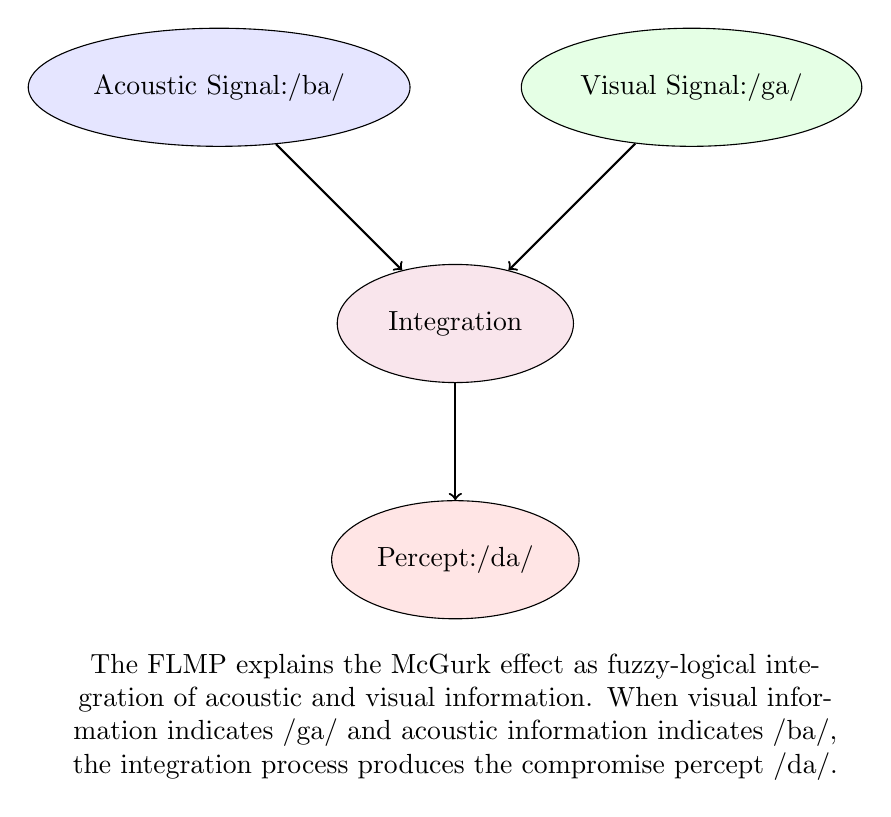
\begin{tikzpicture}
    \node[draw, ellipse, fill=blue!10, minimum width=3cm, minimum height=1.5cm] (acoustic) at (0,0) {Acoustic Signal:\\/ba/};
    
    \node[draw, ellipse, fill=green!10, minimum width=3cm, minimum height=1.5cm] (visual) at (6,0) {Visual Signal:\\/ga/};
    
    \node[draw, ellipse, fill=purple!10, minimum width=3cm, minimum height=1.5cm] (integration) at (3,-3) {Integration};
    
    \node[draw, ellipse, fill=red!10, minimum width=3cm, minimum height=1.5cm] (percept) at (3,-6) {Percept:\\/da/};
    
    \draw[->, thick] (acoustic) -- (integration);
    \draw[->, thick] (visual) -- (integration);
    \draw[->, thick] (integration) -- (percept);
    
    \node[text width=10cm, align=center] at (3,-8) {The FLMP explains the McGurk effect as fuzzy-logical integration of acoustic and visual information. When visual information indicates /ga/ and acoustic information indicates /ba/, the integration process produces the compromise percept /da/.};
\end{tikzpicture}
\end{center}
\end{tcolorbox}

The FLMP shares with TRACE an emphasis on multiple information sources, but differs in several important ways:

\begin{enumerate}
\item \textbf{Representation Format} - While TRACE uses localist representations with activation values, FLMP uses fuzzy truth values that represent degrees of match between input and prototypes.

\item \textbf{Integration Mechanism} - TRACE uses interactive activation with feedback and competition, while FLMP uses fuzzy logical rules to integrate information.

\item \textbf{Developmental Account} - FLMP emphasizes how prototype representations are learned from experience, while TRACE focused less on learning mechanisms.
\end{enumerate}

\subsection{Contemporary Approaches: Prediction and Probabilistic Inference}

Recent approaches to speech perception have increasingly emphasized the role of prediction and probabilistic inference. These frameworks view perception not as passive reception but as active construction based on prior knowledge and incoming sensory information.

\begin{tcolorbox}[enhanced, colback=blue!5, colframe=blue!75!black, title=Predictive Processing in Speech Perception]
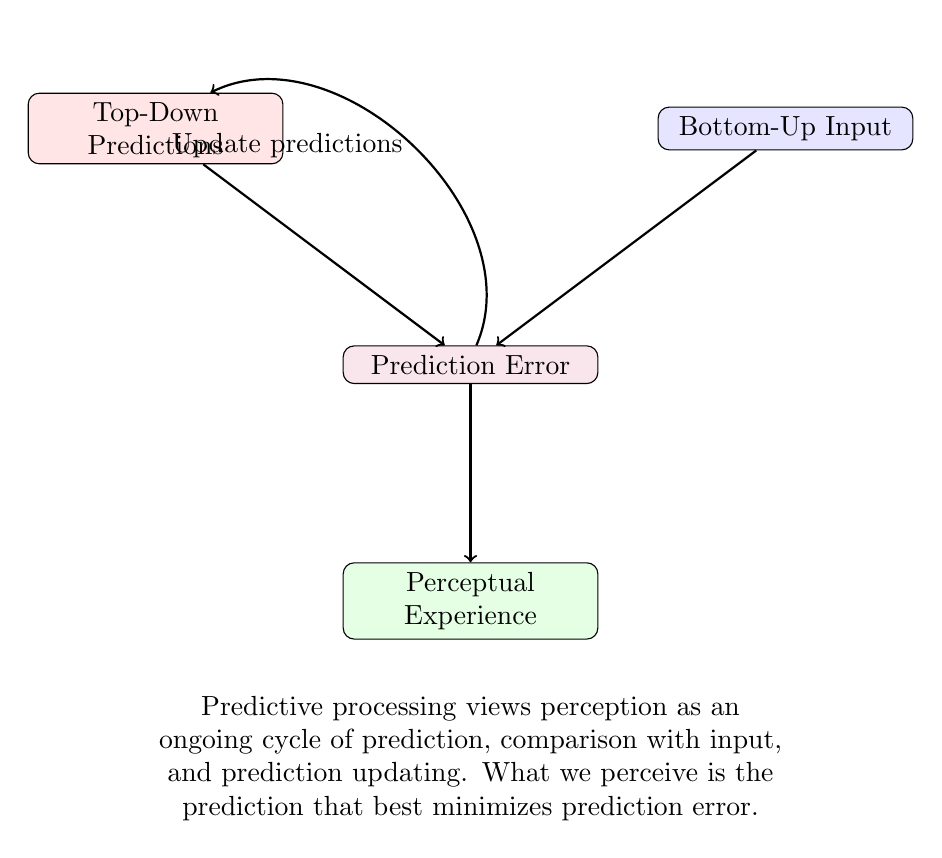
\begin{tikzpicture}
    \node[draw, rectangle, rounded corners, fill=red!10, text width=3cm, align=center] (predictions) at (0,0) {Top-Down Predictions};
    
    \node[draw, rectangle, rounded corners, fill=blue!10, text width=3cm, align=center] (input) at (8,0) {Bottom-Up Input};
    
    \node[draw, rectangle, rounded corners, fill=purple!10, text width=3cm, align=center] (error) at (4,-3) {Prediction Error};
    
    \node[draw, rectangle, rounded corners, fill=green!10, text width=3cm, align=center] (perception) at (4,-6) {Perceptual Experience};
    
    \draw[->, thick] (predictions) -- (error);
    \draw[->, thick] (input) -- (error);
    \draw[->, thick] (error) -- (perception);
    \draw[->, thick, bend right=70] (error) to node[left] {Update predictions} (predictions);
    
    \node[text width=8cm, align=center] at (4,-8) {Predictive processing views perception as an ongoing cycle of prediction, comparison with input, and prediction updating. What we perceive is the prediction that best minimizes prediction error.};
\end{tikzpicture}
\end{tcolorbox}

This predictive framework has several compelling features:

\begin{enumerate}
\item \textbf{Unified Account} - It provides a common mechanism for explaining effects at multiple levels, from phonetic categorization to sentence comprehension.

\item \textbf{Noise Resilience} - Strong predictions allow accurate perception even when acoustic information is degraded or ambiguous, explaining phenomena like phonemic restoration.

\item \textbf{Attention Effects} - The framework naturally accounts for how attention modulates perception by influencing the precision (weight) given to prediction errors.

\item \textbf{Individual Differences} - Differences in prior knowledge and prediction mechanisms can explain individual variations in speech perception.
\end{enumerate}

These predictive approaches have been implemented in computational models that demonstrate how Bayesian inference can account for many speech perception phenomena, including categorical perception, context effects, and adaptation to novel accents.

\begin{figure}[h]
\centering
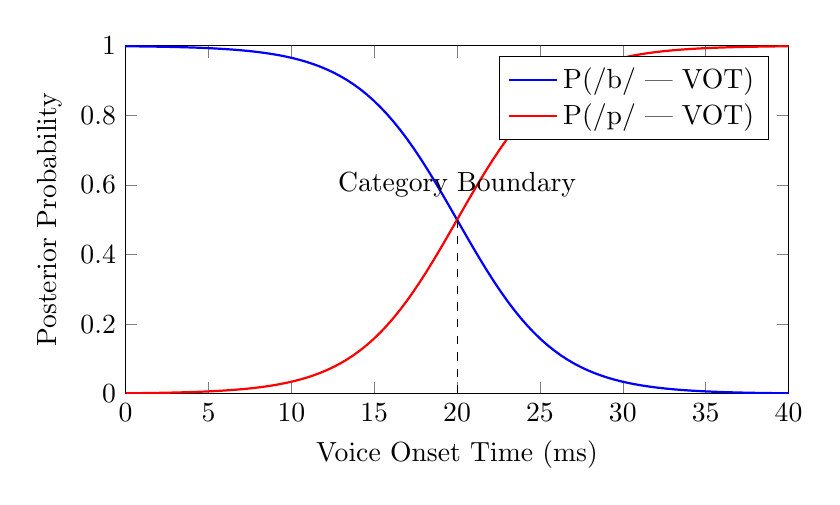
\begin{tikzpicture}
    \begin{axis}[
        width=10cm,
        height=6cm,
        xlabel=Voice Onset Time (ms),
        ylabel=Posterior Probability,
        xmin=0, xmax=40,
        ymin=0, ymax=1,
        legend pos=north east,
        samples=100,
    ]
    
    \addplot[color=blue, thick, domain=0:40] {1/(1+exp((x-20)/3))};
    \addlegendentry{P(/b/ | VOT)}
    
    \addplot[color=red, thick, domain=0:40] {1/(1+exp(-(x-20)/3))};
    \addlegendentry{P(/p/ | VOT)}
    
    \draw[dashed] (axis cs:20,0) -- (axis cs:20,0.5);
    \node at (axis cs:20,0.6) {Category Boundary};
    
    \end{axis}
\end{tikzpicture}
\caption{Bayesian categorization of speech sounds based on voice onset time}
\label{fig:bayesian_vot}
\end{figure}

The Bayesian approach frames speech perception as inferring the most likely linguistic units (phonemes, words, meanings) given the acoustic evidence and prior knowledge. This naturally incorporates both bottom-up and top-down information in a mathematically principled way.

\subsection{Neural Implementations: From Specialized Modules to Distributed Networks}

Our understanding of the neural basis of speech perception has evolved alongside theoretical models. Early neuroanatomical models based on lesion studies proposed specialized modules for speech perception (Wernicke's area) and production (Broca's area).

\begin{figure}[h]
\centering
\begin{tikzpicture}
    \node[inner sep=0pt] (brain) at (0,0) {\includegraphics[width=6cm]{brain}};
    
    \node[draw, ellipse, fill=green!20, minimum width=2cm, minimum height=1cm] (wernicke) at (2,0.5) {Wernicke's Area};
    \node[draw, ellipse, fill=red!20, minimum width=2cm, minimum height=1cm] (broca) at (-2,-0.5) {Broca's Area};
    
    \node[text width=3cm, align=center] at (3.5,2) {Classical model:\\Specialized areas for perception and production};
\end{tikzpicture}
\caption{Classical neuroanatomical model of language areas}
\label{fig:classical_brain}
\end{figure}

Modern neuroimaging has revealed a much more complex and distributed network for speech perception, with multiple parallel pathways and extensive interaction between traditionally "perceptual" and "motor" regions.

\begin{tcolorbox}[enhanced, colback=purple!5, colframe=purple!75!black, title=Distributed Neural Networks for Speech Perception]
\begin{center}
\begin{tikzpicture}
    \node[inner sep=0pt] (brain) at (0,0) {\includegraphics[width=8cm]{brain_network}};
    
    \node[draw, ellipse, fill=red!10, minimum width=1.5cm, minimum height=0.8cm] (stg) at (2,1) {STG};
    \node[draw, ellipse, fill=blue!10, minimum width=1.5cm, minimum height=0.8cm] (ips) at (0,2) {IPS};
    \node[draw, ellipse, fill=green!10, minimum width=1.5cm, minimum height=0.8cm] (ifg) at (-2,0) {IFG};
    \node[draw, ellipse, fill=yellow!10, minimum width=1.5cm, minimum height=0.8cm] (mtg) at (0,-2) {MTG};
    
    \draw[<->, thick] (stg) -- (ips);
    \draw[<->, thick] (stg) -- (ifg);
    \draw[<->, thick] (stg) -- (mtg);
    \draw[<->, thick] (ips) -- (ifg);
    \draw[<->, thick] (ifg) -- (mtg);
    \draw[<->, thick] (mtg) -- (ips);
    
    \node[text width=8cm, align=center] at (0,-4) {Modern view: Speech perception involves distributed networks with extensive interaction between auditory, motor, and semantic processing regions. STG = Superior Temporal Gyrus, IPS = Intraparietal Sulcus, IFG = Inferior Frontal Gyrus, MTG = Middle Temporal Gyrus.};
\end{tikzpicture}
\end{center}
\end{tcolorbox}

This distributed network perspective helps reconcile seemingly contradictory findings:

\begin{enumerate}
\item It explains why motor regions (Broca's area and motor cortex) activate during speech perception tasks, as noted in studies supporting motor theory.

\item It accounts for why patients with motor speech disorders can still comprehend speech, as multiple pathways can support perception.

\item It accommodates findings that non-human animals without speech production capabilities can discriminate speech sounds, as auditory pathways may be sufficient for many aspects of speech perception.
\end{enumerate}

The distributed network view aligns with modern computational approaches that emphasize parallel processing and integration of multiple information sources—a far cry from the modular, sequential processing assumed in early models.

\section{Unified Perspectives: Toward a Comprehensive Theory of Speech Perception}

The evolution from specialized models like TRACE to general frameworks like Shannon-Weaver and finally to integrative approaches reveals a trajectory toward increasingly comprehensive theories of speech perception. Modern theories attempt to unify insights from multiple traditions while addressing the limitations of earlier approaches.

\subsection{Common Principles Across Theories}

Despite their differences, contemporary theories of speech perception converge on several key principles:

\begin{tcolorbox}[enhanced, colback=green!5, colframe=green!75!black, title=Converging Principles in Modern Speech Perception Theories]
\begin{enumerate}
\item \textbf{Multiple Information Sources} - Speech perception integrates acoustic information with linguistic knowledge, visual cues, and contextual factors.

\item \textbf{Bidirectional Processing} - Information flows both bottom-up and top-down, with continuous interaction between levels.

\item \textbf{Probabilistic Inference} - Perception involves weighing evidence and prior knowledge to reach the most likely interpretation.

\item \textbf{Distributed Neural Implementation} - Speech perception engages widespread brain networks rather than isolated modules.

\item \textbf{Learning and Adaptation} - Perceptual mechanisms adapt to new speakers, accents, and acoustic environments through experience.
\end{enumerate}
\end{tcolorbox}

These common principles provide a foundation for developing unified theories that can explain the remarkable flexibility and robustness of human speech perception.

\subsection{Remaining Debates and Open Questions}

Despite this convergence, several fundamental debates remain unresolved:

\begin{enumerate}
\item \textbf{The Role of Motor Representations} - To what extent are motor representations necessary for speech perception? The evidence remains mixed, with some studies showing motor involvement and others suggesting auditory representations may be sufficient.

\item \textbf{Domain Specificity} - Is speech perception accomplished by specialized mechanisms evolved for language, or does it rely on general auditory and cognitive processes? This debate continues to influence research and theory.

\item \textbf{The Unit of Perception} - What are the basic units that listeners extract from the speech signal? Possibilities include features, phonemes, syllables, gestures, or exemplars of whole words.

\item \textbf{Individual Differences} - How and why do individuals differ in speech perception abilities, and what factors (cognitive, developmental, experiential) explain these differences?
\end{enumerate}

\begin{figure}[h]
\centering
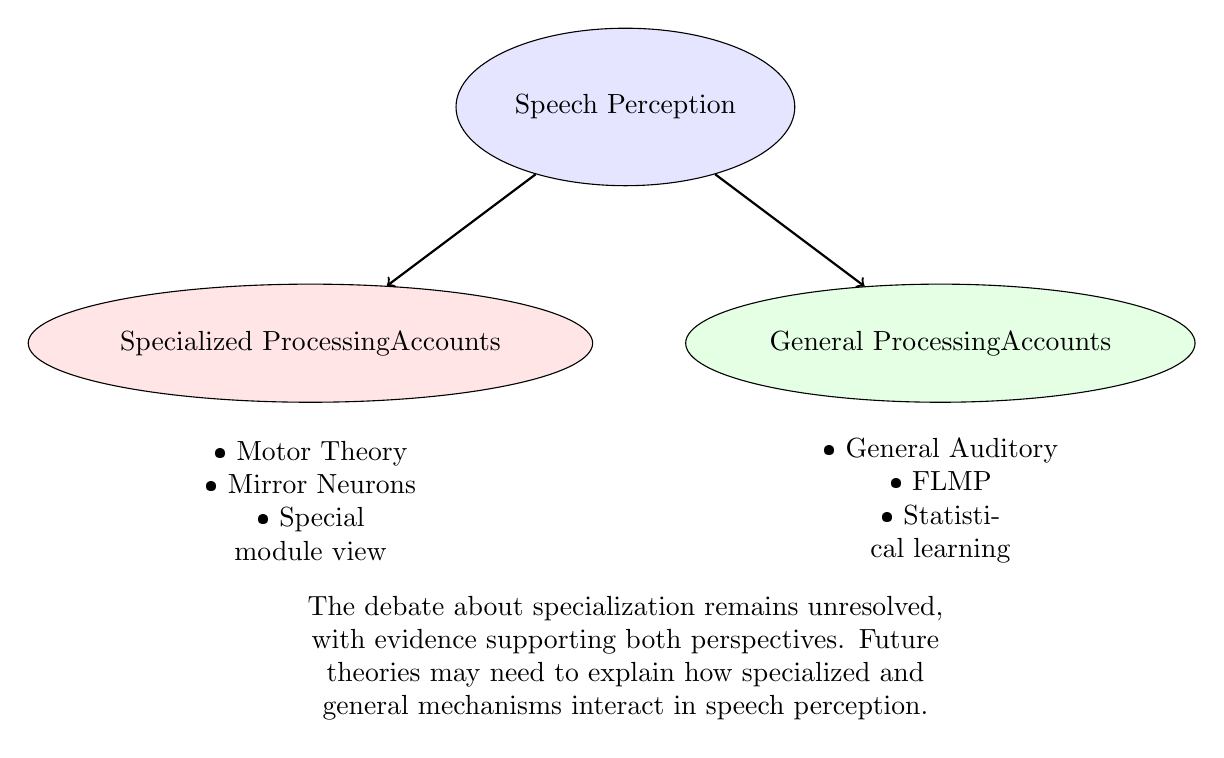
\begin{tikzpicture}
    \node[draw, ellipse, fill=blue!10, minimum width=4cm, minimum height=2cm] (speech) at (0,0) {Speech Perception};
    
    \node[draw, ellipse, fill=red!10, minimum width=3cm, minimum height=1.5cm] (specialized) at (-4,-3) {Specialized Processing\\Accounts};
    \node[draw, ellipse, fill=green!10, minimum width=3cm, minimum height=1.5cm] (general) at (4,-3) {General Processing\\Accounts};
    
    \draw[->, thick] (speech) -- (specialized);
    \draw[->, thick] (speech) -- (general);
    
    \node[text width=3cm, align=center] at (-4,-5) {• Motor Theory\\• Mirror Neurons\\• Special module view};
    \node[text width=3cm, align=center] at (4,-5) {• General Auditory\\• FLMP\\• Statistical learning};
    
    \node[text width=10cm, align=center] at (0,-7) {The debate about specialization remains unresolved, with evidence supporting both perspectives. Future theories may need to explain how specialized and general mechanisms interact in speech perception.};
\end{tikzpicture}
\caption{Ongoing debate about specialized versus general processing in speech perception}
\label{fig:specialization_debate}
\end{figure}

These debates reflect deeper philosophical questions about modularity, embodiment, and the relationship between perception and action. As philosopher Alva Noë has argued, perception may be neither purely specialized nor purely general, but rather a skilled activity that develops through interaction with the environment.

\subsection{Practical Applications: From Theory to Technology}

The evolution of speech perception theories has profoundly influenced speech technology, from automatic speech recognition to hearing aids and cochlear implants.

\begin{table}[h]
\centering
\begin{tabular}{|p{4cm}|p{8cm}|}
\hline
\textbf{Application} & \textbf{Theoretical Influence} \\
\hline
Automatic Speech Recognition & TRACE-inspired recurrent networks capture temporal dependencies; Bayesian approaches incorporate predictive processing principles \\
\hline
Hearing Aids & FLMP insights about multimodal integration inform designs that combine acoustic with visual cues \\
\hline
Cochlear Implants & Understanding of redundancy in speech guides channel allocation and signal processing strategies \\
\hline
Second Language Learning & Findings about perceptual learning and adaptation shape training programs for non-native speech perception \\
\hline
\end{tabular}
\caption{Theoretical influences on practical applications}
\label{tbl:applications}
\end{table}

The most successful applications typically incorporate principles from multiple theoretical traditions, much as unified theories attempt to integrate insights from diverse research programs.

\subsection{Future Directions: Beyond Traditional Frameworks}

The future of speech perception research likely lies in transcending traditional theoretical boundaries to develop frameworks that can explain not just how we perceive isolated utterances in controlled laboratory settings, but how we engage in real-world communication.

\begin{tcolorbox}[enhanced, colback=yellow!5, colframe=yellow!75!black, title=Emerging Research Directions]
\begin{enumerate}
\item \textbf{Social and Pragmatic Factors} - How social relationships, communicative intentions, and pragmatic context influence speech perception

\item \textbf{Multimodal Integration} - How speech perception integrates with gesture, facial expression, and other communicative channels

\item \textbf{Variability and Adaptation} - How listeners adapt to different speakers, accents, and acoustic environments

\item \textbf{Developmental Trajectories} - How speech perception develops from infancy through adulthood, and how early experience shapes perception

\item \textbf{Cultural and Linguistic Diversity} - How speech perception mechanisms vary across languages and cultures
\end{enumerate}
\end{tcolorbox}

These emerging directions reflect a broader shift from studying speech perception as an isolated cognitive process to understanding it as part of situated, embodied, and socially embedded communication.

\section{Conclusion: The Integrated Nature of Speech Processing}

From the specialized temporal processing of TRACE to the general communicative framework of Shannon-Weaver, our understanding of speech perception has evolved toward increasingly sophisticated accounts that recognize the dynamic, interactive nature of how we extract meaning from the speech signal. This evolution reflects both theoretical advances within cognitive science and practical developments in technology and clinical applications.

Contemporary perspectives emphasize that speech perception is neither a purely bottom-up analysis of acoustic signals nor a top-down construction based on expectations, but rather a complex interplay between multiple sources of information at different levels. The remarkable robustness of human speech perception—our ability to understand speech in noisy environments, adapt to unfamiliar accents, and integrate information across sensory modalities—stems from this integrative nature.

As we continue to investigate the mechanisms underlying speech perception, we move closer to understanding one of humanity's most remarkable achievements: the ability to transform patterns of air pressure variations into meaningful linguistic experiences. This understanding not only illuminates fundamental aspects of human cognition but also guides the development of technologies that improve communication for all people.

The journey from specialized to integrated models reminds us that progress in science often involves not just accumulating facts but reconceptualizing the phenomena we study—seeing familiar processes in new ways that reveal previously hidden connections and possibilities. By embracing the complexity of speech perception rather than reducing it to isolated components, we gain deeper insight into the extraordinary human capacity for language.

\end{document}